% ============================================
% DOCUMENT PRINCIPAL - Projet de Fin d'Études
% ============================================
% Ce fichier est le SEUL que vous devez modifier tout au long de l'année.
% Instructions:
% - Modifiez ce fichier pour ajouter votre contenu
% - Ajoutez vos références dans references.bib
% - NE PAS MODIFIER preamble.tex sauf si vous avez besoin d'ajouter des packages spécifiques
%
% Compilation: pdflatex main.tex (2 fois) puis bibtex main puis pdflatex main.tex
% ============================================


% Charger le préambule avec tous les packages
% DO NOT COMPILE THIS FILE DIRECTLY. Compile main.tex instead.
% ============================================
% PRÉAMBULE - Configuration LaTeX du Projet
% ============================================
% Ce fichier contient tous les packages et configurations LaTeX.
% NE PAS MODIFIER CE FICHIER sauf si vous avez besoin d'ajouter des packages spécifiques.
% Modifiez uniquement main.tex pour votre contenu.

\documentclass[12pt]{report}

% ============================================
% MISE EN PAGE
% ============================================% Düzeltilmiş satır:
\usepackage[a4paper, margin=2cm, marginparwidth=0pt, top=2cm]{geometry}

% ============================================
% PACKAGES GRAPHIQUES ET FIGURES
% ============================================
\usepackage[pdftex]{graphicx}
\usepackage{subcaption}
\usepackage{color}
\usepackage{xcolor}
\usepackage{float}

% ============================================
% PACKAGES POUR LE CODE SOURCE
% ============================================
\usepackage{listings}

% ============================================
% PACKAGES MATHÉMATIQUES
% ============================================
\usepackage{amsmath, amsfonts, amssymb, amsthm}

% ============================================
% ENCODAGE ET POLICE
% ============================================
\usepackage{libertine}
\usepackage[utf8]{inputenc}
\usepackage[T1]{fontenc}

% ============================================
% HYPERLIENS ET RÉFÉRENCES
% ============================================
\usepackage{hyperref}
\usepackage[normalem]{ulem}

\usepackage{listings}
\usepackage{xcolor}

\lstset{
    language=Python,
    basicstyle=\ttfamily\small,
    keywordstyle=\color{blue},
    stringstyle=\color{red},
    commentstyle=\color{green!60!black},
    numbers=left,
    numberstyle=\tiny\color{gray},
    stepnumber=1,
    numbersep=5pt,
    backgroundcolor=\color{gray!5},
    frame=single,
    rulecolor=\color{black!30},
    breaklines=true,
    captionpos=b,
    escapeinside={(*@}{@*)} % LaTeX formülleri kod içine gömmek için
}
% ============================================
% INDENTATION ET TITRES
% ============================================
\usepackage{indentfirst}
\usepackage{titlesec}
\titleformat{\chapter}[display]
  {\normalfont\huge\bfseries}{}{0pt}{\Huge}
\titlespacing*{\chapter}{0pt}{10pt}{20pt}

\setcounter{secnumdepth}{3}

% ============================================
% COMMANDES PERSONNALISÉES
% ============================================
% Commande pour mettre du texte en rouge (notes)
\newcommand{\nt}[1]{\textcolor{red}{#1}}

% Ligne horizontale
\newcommand{\HRule}{\rule{\linewidth}{0.5mm}}

% ============================================
% ENVIRONNEMENTS MATHÉMATIQUES
% ============================================
\newtheorem{theorem}{Th\'{e}or\`{e}me}
\newtheorem{lemma}[theorem]{Lemme}
\newtheorem{proposition}[theorem]{Proposition}
\newtheorem{corollary}[theorem]{Corollaire}

\newtheorem{definition}{D\'{e}finition}
\newtheorem{conjecture}{Conjecture}
\newtheorem{example}{Exemple}
\newtheorem{remark}{Remarque}

\def\proofname{D\'emonstration}

% ============================================
% COMMANDES MATHÉMATIQUES PERSONNALISÉES
% ============================================
\newcommand{\N}{\mathbf{N}}     % Entiers naturels
\newcommand{\R}{\mathbf{R}}     % Réels
\newcommand{\C}{\mathbf{C}}     % Complexes
\newcommand{\Z}{\mathbf{Z}}     % Entiers relatifs
\newcommand{\Q}{\mathbf{Q}}     % Rationnels

% ============================================
% RENOMMAGE DES SECTIONS
% ============================================
\renewcommand*\contentsname{Table des Matières}
\renewcommand*\bibname{Références}

\usepackage{listings}
\usepackage{xcolor}

% Renk tanımlamaları
\definecolor{codegreen}{rgb}{0,0.6,0}
\definecolor{codegray}{rgb}{0.5,0.5,0.5}
\definecolor{codepurple}{rgb}{0.58,0,0.82}
\definecolor{backcolour}{rgb}{0.95,0.95,0.92}

% Python stil ayarları
\lstset{
    language=Python,
    backgroundcolor=\color{backcolour},
    commentstyle=\color{codegreen},
    keywordstyle=\color{magenta},
    numberstyle=\tiny\color{codegray},
    stringstyle=\color{codepurple},
    basicstyle=\ttfamily\small,
    breakatwhitespace=false,
    breaklines=true,
    captionpos=b,
    keepspaces=true,
    numbers=left,
    numbersep=5pt,
    showspaces=false,
    showstringspaces=false,
    showtabs=false,
    tabsize=2,
    frame=single
    language=Python,
    basicstyle=\ttfamily\small,
    keywordstyle=\color{blue!70!black},
    stringstyle=\color{red!70!black},
    commentstyle=\color{gray},
    frame=single,
    breaklines=true,
    numbers=left,
    numberstyle=\tiny\color{gray},
    showstringspaces=false
    language=Python,
    basicstyle=\ttfamily\small,
    keywordstyle=\color{blue!70!black},
    stringstyle=\color{red!70!black},
    commentstyle=\color{green!50!black},
    frame=single,
    breaklines=true,
    numbers=left,
    numberstyle=\tiny\color{gray},
    showstringspaces=false,
    tabsize=4,
    extendedchars=true,
}

\begin{document}

% ============================================
% PAGE DE TITRE
% ============================================
\begin{titlepage}

    \begin{center}

        
\includegraphics[width=0.15\textwidth]{logoGSU.png}\\[1cm]

        \addtolength{\voffset}{-1cm}
        \addtolength{\textheight}{2cm}

        \hspace{-3cm}

        \large{\textbf{PROJET DE FIN D'\'ETUDES}}

        \vspace{0.5cm}

        {\small pour obtenir le diplôme de}

        \vspace{0.5cm}

        l'\,\textsc{\textbf{Université Galatasaray}}

        {\small Spécialité : \textbf{Mathématiques}}\\

        \vspace{0.75cm}

        \vspace{1.5cm}

        % ⚠️ MODIFIEZ ICI: Votre titre
        {\Large\textbf{{Approximation de Matrices de Rang Faible pour la Compression d'Images avec la DVS}}}

        \vspace{0.25cm}

        % ⚠️ MODIFIEZ ICI: Le numéro du rapport (Rapport 1, Rapport 2, Rapport 3, ou Mémoire Final)
        %{Rapport 1 }

        \vspace{1.25cm}

        % ⚠️ MODIFIEZ ICI: Votre nom
        \normalsize \textrm{Préparé par : } \textbf{BERRİN KARAKAYA}

        % ⚠️ MODIFIEZ ICI: Le nom du responsable
        \small Résponsable : \textbf{OĞUZHAN KAYA}

        \vspace{2.50cm}

        % ⚠️ MODIFIEZ ICI: La date
        %\emph{{{07/10/2025}}}

    \end{center}

\end{titlepage}

% ============================================
% NUMÉROTATION ROMAINE POUR LES PRÉLIMINAIRES
% ============================================
\pagenumbering{roman}

% ============================================
% TABLE DES MATIÈRES
% ============================================
\tableofcontents
\clearpage

% ============================================
% DÉBUT DU CONTENU PRINCIPAL
% ============================================
\pagenumbering{arabic}


% ============================================
% SECTIONS PRINCIPALES
% ============================================
% ⚠️ MODIFIEZ ICI: Ajoutez votre contenu ci-dessous
% Pour Rapport 1: Objectifs, Résultats Préliminaires, Prochaines étapes
% Pour Rapport 2-3: Ajoutez Introduction et développez les sections
% Pour Mémoire Final: Structure complète avec Introduction, Chapitres, Conclusion

\section*{Objectifs du Projet}
\addcontentsline{toc}{section}{Objectifs du Projet}
Dans ce projet, nous étudions comment les outils de la Théorème Spectral peuvent être utilisés pour analyser des matrices de grande dimension. L’objectif est de comprendre comment obtenir une approximation de rang faible d'une image numérique (représentée par une matrice), tout en minimisant la perte d'information par rapport à la représentation initiale.

Dans un premier temps, nous rappelons les notions de base de la Théorème Spectral. Nous montrons ensuite comment cette approche conduit à la décomposition en valeurs singulières dans le cas des matrices rectangulaires.

Enfin, nous appliquons ces outils à des images numériques afin de construire des approximations de ces images en utilisant une quantité réduite de données. Ce travail permet d’illustrer, d’un point de vue mathématique, comment la Décomposition en Valeurs Singulières conduit à une réduction de dimension.

\section*{Introduction}
\addcontentsline{toc}{section}{Introduction}

Comprendre une application linéaire peut être difficile, car la matrice qui la représente peut contenir plusieurs effets géométriques dans des espaces de grande dimension. Le Théorème Spectral nous aide à comprendre ces transformations d’une manière simple. Il montre qu’une matrice symétrique peut être écrite avec des vecteurs propres et des valeurs propres. Les valeurs propres indiquent combien la transformation agrandit ou réduit dans une direction. Les vecteurs propres sont des vecteurs dont la direction ne change pas sous cette transformation. Ainsi, la transformation devient plus claire. Les matrices orthogonales sont utiles car elles gardent les distances et les angles. Elles représentent des rotations ou des symétries. Elles ne déforment pas l’espace et sont très stables dans les calculs, ce qui est important en informatique. La matrice diagonale obtenue avec les valeurs propres permet de simplifier les calculs. Les calculs de puissance ou l'inverse d'une telle matrice sont plus faciles.

Cependant, dans de nombreuses applications, les objets étudiés ne sont pas représentés par des matrices carrées ou symétriques. Pour traiter ce type de matrices, on peut construire des matrices symétriques associées, comme $A^\top A$ , auxquelles le Théorème Spectral peut être appliqué. Cette approche conduit naturellement à la Décomposition en Valeurs Singulières, qui étend la notion de diagonalisation au cas des matrices rectangulaires. La décomposition en valeurs singulières permet d’écrire une matrice comme une somme de matrices de rang 1. La Décomposition en Valeurs Singulières permet de représenter la matrice associée à l’image originale à l’aide d’une quantité réduite d’informations, tout en restant proche de la matrice initiale. Cette démarche s’inscrit dans le cadre de l’approximation de matrices et conduit à une réduction de dimension, puisque l’image est décrite avec moins d’informations que dans sa représentation initiale.

Dans cette thèse, nous étudierons la Théorème Spectral, la Décomposition en Valeurs Singulières et l'approximation matricielle. En appliquant ces outils aux images numériques, nous démontrerons comment on peut approximer à une image peut être représentée par une matrice par des matrices d'ordre inférieur. L'objectif de ce travail est de fournir une compréhension mathématique claire de la manière dont la réduction de dimensionnalité peut être obtenue à partir de la structure des matrices associées aux images.


\clearpage

\subsection*{Théorème Spectral}
\addcontentsline{toc}{section}{Théorème Spectral}
\noindent Le Théorème Spectral permet de représenter l'application linéaire $T : \mathbb{R}^n \to \mathbb{R}^n$ associée à $A \in \mathbb{R}^{n \times n}$ une matrice symétrique réelle si et seulement si $A$ peut être exprimée sous la forme :
\[
    A = QDQ^{\top}
\]
où $Q$ est une {matrice orthogonale} dont les colonnes $\{u_1, \dots, u_n\}$ sont les {vecteurs propres} de $A$. Ces colonnes forment une base orthonormale pour $\mathbb{R}^n$. Puisque $Q$ est orthogonal, son inverse est égal à sa transposée, ${Q^{-1} = Q^{\top}}$.

\noindent $D$ est une {matrice diagonale} dont les éléments diagonaux sont les {valeurs propres} de $A$, correspondant aux vecteurs propres dans $Q$ dans le même ordre.

\noindent Autrement dit, on peut écrire la matrice $A$ simplement comme une somme de ses valeurs propres et vecteurs propres :
\[
    A = \lambda_1 u_1 u_1^\top + \lambda_2 u_2 u_2^\top + \dots + \lambda_n u_n u_n^\top = \sum_{i=1}^{n} \lambda_i u_i u_i^\top.
\]

\begin{example}

    Considérons la matrice symétrique $A\in \mathbb{R}^{3 \times 3}$ suivante :
    \[
        A =
        \begin{pmatrix}
            2 & 0 & 0 \\
            0 & 3 & 1 \\
            0 & 1 & 3
        \end{pmatrix}.
    \]
\end{example}
\noindent Tout d'abord on détermine $\operatorname{spec}(A)$.
Le polynôme caractéristique est
\[
    \det(A - \lambda I) =
    \det
    \begin{pmatrix}
        2-\lambda & 0         & 0         \\
        0         & 3-\lambda & 1         \\
        0         & 1         & 3-\lambda
    \end{pmatrix} = 0.
\]
On obtient :
\[
    (2-\lambda)((3-\lambda)^2 - 1) = 0 \implies (2-\lambda)(2-\lambda)(4-\lambda) = 0 \implies (2-\lambda)^2 (4-\lambda) = 0.
\]
Ainsi, l'ensemble des valeurs propres est $\operatorname{spec}(A)$ = \{2, 4\}.
Ensuite, on trouve les vecteurs $v$ non-nuls qui satisfait $(A - \lambda I)v = 0$.

\noindent Pour $\lambda = 2$:
\[
    (A - 2I)v = 0 \implies
    \begin{pmatrix} 0 & 0 & 0 \\ 0 & 1 & 1 \\ 0 & 1 & 1 \end{pmatrix}
    \begin{pmatrix}x\\y\\z\end{pmatrix} =
    \begin{pmatrix}0\\0\\0\end{pmatrix} \implies y + z = 0.
\]

\noindent Les vecteurs de base sont : $v_1 = \begin{pmatrix}1\\0\\0\end{pmatrix}, \quad v_2 = \begin{pmatrix}0\\1\\-1\end{pmatrix}.$

\noindent Pour $\lambda = 4$:
\[
    (A - 4I)v = 0 \implies
    \begin{pmatrix} -2 & 0 & 0 \\ 0 & -1 & 1 \\ 0 & 1 & -1 \end{pmatrix}
    \begin{pmatrix}x\\y\\z\end{pmatrix} =
    \begin{pmatrix}0\\0\\0\end{pmatrix} \implies y=z.
\]
Le vecteur de base est : $v_3 = \begin{pmatrix}0\\1\\1\end{pmatrix}.$
\[
\]
\noindent On va écrire une matrice orthogonale $Q$ . Cela signifie que les vecteurs propres que nous plaçons dans $Q$ peuvent être et {orthogonaux} entre eux. Ainsi, si un vecteur propre n'est pas de longueur 1, nous le normalisons en le divisant par sa norme $\|v\|$ : Nous normalisons les vecteurs $v$ en $u = v/\|v\|$:
\[
    u_1 = \frac{v_1}{\|v_1\|} = \frac{1}{1} \begin{pmatrix}1\\0\\0\end{pmatrix} = \begin{pmatrix}1\\0\\0\end{pmatrix}
\]
\[
    u_2 = \frac{v_2}{\|v_2\|} = \frac{1}{\sqrt{0^2+1^2+(-1)^2}} \begin{pmatrix}0\\1\\-1\end{pmatrix} = \begin{pmatrix}0\\1/\sqrt{2}\\-1/\sqrt{2}\end{pmatrix}
\]
\[
    u_3 = \frac{v_3}{\|v_3\|} = \frac{1}{\sqrt{0^2+1^2+1^2}} \begin{pmatrix}0\\1\\1\end{pmatrix} = \begin{pmatrix}0\\1/\sqrt{2}\\1/\sqrt{2}\end{pmatrix}
\]
\noindent $Q$ est la matrice {orthogonale} formée des vecteurs propres normalisés $\{u_1, u_2, u_3\}$:
\[
    Q = [u_1 \; u_2 \; u_3] =
    \begin{pmatrix}
        1 & 0           & 0          \\
        0 & 1/\sqrt{2}  & 1/\sqrt{2} \\
        0 & -1/\sqrt{2} & 1/\sqrt{2}
    \end{pmatrix}.
\]

\noindent $D$ est la {matrice diagonale} des valeurs propres correspondantes:
\[
    D = \text{diag}(2, 2, 4) =
    \begin{pmatrix}
        2 & 0 & 0 \\
        0 & 2 & 0 \\
        0 & 0 & 4
    \end{pmatrix}.
\]
Le Théorème Spectral est vérifié :
\[
    \boxed{A = Q D Q^{\top}}
\]

\begin{lemma}[Valeurs propres réelles]
    Toutes les valeurs propres d'une matrice symétrique réelle sont réelles.
\end{lemma}

\begin{proof}
    Soit $\lambda \in \mathbb{C}$ une valeur propre de la matrice réelle symétrique $A$ et $x \in \mathbb{C}^n$ un vecteur propre associé non nul ($x \neq 0$), tel que $Ax = \lambda x$.

    \noindent On considère $\mathbb{C}^n$ muni du produit scalaire hermitien usuel noté $\langle \cdot, \cdot \rangle$.
    Puisque $A$ est réelle et symétrique ($A = A^\top$), on a $A = \overline{A}^\top = A^*$.

    \noindent Par la propriété de l'adjoint dans un produit scalaire ($\langle Ax, y \rangle = \langle x, A^* y \rangle$), nous obtenons l'égalité suivante :
    \[
        \langle Ax, x \rangle = \langle x, A^* x \rangle = \langle x, Ax \rangle.
    \]

    \noindent En remplaçant $A x = \lambda x$, on obtient :
    \[
        \langle \lambda x, x \rangle = \langle x, \lambda x \rangle
    \]
    En utilisant les propriétés de linéarité du produit scalaire :
    \[
        \lambda \langle x, x \rangle = \bar{\lambda} \langle x, x \rangle
    \]
    Comme $x \neq 0$, on a $\langle x, x \rangle = \|x\|^2 > 0$. Nous pouvons donc simplifier l'équation :
    \[
        \lambda = \bar{\lambda}
    \]
    Ceci implique que la partie imaginaire de $\lambda$ est nulle, donc $\lambda \in \mathbb{R}$.
\end{proof}

\begin{lemma}[Vecteurs propres orthogonaux]
    Les vecteurs propres correspondant à des valeurs propres distinctes d'une matrice symétrique sont orthogonaux.
\end{lemma}

\begin{proof}
    Soient $\lambda_1$ et $\lambda_2$ deux valeurs propres distinctes correspondant respectivement aux vecteurs propres $x_1$ et $x_2$, tels que $Ax_1 = \lambda_1 x_1$ et $Ax_2 = \lambda_2 x_2$.

    \noindent Nous allons établir deux égalités pour comparer les produits scalaires.
    \noindent Prenons la première équation $Ax_1 = \lambda_1 x_1$. Appliquons d'abord la transposée des deux côtés, puis multiplions à droite par le vecteur $x_2$ :
    \[
        (A x_1)^\top = (\lambda_1 x_1)^\top \implies x_1^\top A^\top = \lambda_1 x_1^\top
    \]
    Puisque $A$ est symétrique ($A = A^\top$), on remplace $A^\top$ par $A$. En multipliant ensuite à droite par $x_2$, on obtient :
    \[
        x_1^\top A x_2 = \lambda_1 x_1^\top x_2
    \]

    \noindent Partons maintenant de la deuxième équation $Ax_2 = \lambda_2 x_2$. Cette fois, multiplions directement à gauche par le vecteur transposé $x_1^\top$ :
    \[
        x_1^\top (A x_2) = x_1^\top (\lambda_2 x_2) \implies x_1^\top A x_2 = \lambda_2 x_1^\top x_2
    \]

    \noindent En égalisant ces deux expressions, nous obtenons :
    \[
        \lambda_1 x_1^\top x_2 = \lambda_2 x_1^\top x_2
    \]
    Ce qui équivaut à :
    \[
        (\lambda_1 - \lambda_2) x_1^\top x_2 = 0
    \]
    Puisque les valeurs propres sont distinctes ($\lambda_1 \neq \lambda_2$), on a nécessairement $\lambda_1 - \lambda_2 \neq 0$. Par conséquent, le produit scalaire doit être nul :
    \[
        x_1^\top x_2 = 0
    \]
    Cela prouve que les vecteurs propres $x_1$ et $x_2$ sont orthogonaux.
\end{proof}

\begin{lemma}[Indépendance des Vecteurs Propres]
    Si une matrice $A \in \mathbb{R}^{n \times n}$ possède $k$ valeurs propres distinctes, alors tout ensemble de $k$ vecteurs propres correspondants (non nuls) est linéairement indépendant.
\end{lemma}

\begin{proof}
    Nous prouvons ce théorème par récurrence.

    \textbf{Initialisation :} D'abord, montrons que deux vecteurs propres correspondant à des valeurs propres distinctes sont linéairement indépendants. Soient $v_1$ et $v_2$ des vecteurs propres associés respectivement aux valeurs propres distinctes $\lambda_1$ et $\lambda_2$. Supposons, par l'absurde, que $v_1$ et $v_2$ sont linéairement dépendants. Alors il existe deux scalaires $\alpha_1, \alpha_2$ (non tous les deux nuls) tels que:
    \begin{equation} \label{eq:indep1}
        \alpha_1 v_1 + \alpha_2 v_2 = 0
    \end{equation}
    En multipliant (\ref{eq:indep1}) à gauche par $A$, on obtient :
    \begin{equation} \label{eq:indep2}
        \alpha_1 \lambda_1 v_1 + \alpha_2 \lambda_2 v_2 = 0
    \end{equation}
    De même, en multipliant (\ref{eq:indep1}) par $\lambda_2$, on obtient :
    \begin{equation} \label{eq:indep3}
        \alpha_1 \lambda_2 v_1 + \alpha_2 \lambda_2 v_2 = 0
    \end{equation}
    En soustrayant l'équation (\ref{eq:indep2}) de l'équation (\ref{eq:indep3}), on trouve :
    \[
        \alpha_1 (\lambda_2 - \lambda_1) v_1 = 0.
    \]
    Puisque $\lambda_2 \neq \lambda_1$ et $v_1 \neq 0$, nous devons avoir $ \alpha_1 = 0$. Comme $v_2 \neq 0$, en remplaçant $\alpha_1=0$ dans (\ref{eq:indep1}), on obtient $\alpha_2=0$, ce qui mène à une contradiction. Ainsi, $v_1$ et $v_2$ sont linéairement indépendants.

    \textbf{Hérédité :} Supposons maintenant que tout ensemble de $j < k$ vecteurs propres correspondant à des valeurs propres distinctes est linéairement indépendant. Nous voulons montrer que $j+1$ vecteurs propres sont aussi linéairement indépendants.

    \noindent Soient $v_1, v_2, \dots, v_j$ des vecteurs propres linéairement indépendants correspondant à des valeurs propres distinctes $\lambda_1, \lambda_2, \dots, \lambda_j$. Supposons par l'absurde qu'un vecteur propre supplémentaire $v_{j+1}$, correspondant à une valeur propre différente $\lambda_{j+1}$, est linéairement dépendant de $v_1, \dots, v_j$. Alors il existe des scalaires $\alpha_1, \alpha_2, \dots, \alpha_j$ non tous nuls tels que :
    \begin{equation} \label{eq:indep4}
        v_{j+1} = \alpha_1 v_1 + \alpha_2 v_2 + \dots + \alpha_j v_j
    \end{equation}
    En multipliant (\ref{eq:indep4}) à gauche par $A$ :
    \begin{equation} \label{eq:indep5}
        \lambda_{j+1} v_{j+1} = \alpha_1 \lambda_1 v_1 + \alpha_2 \lambda_2 v_2 + \dots + \alpha_j \lambda_j v_j
    \end{equation}
    En multipliant (\ref{eq:indep4}) par le scalaire $\lambda_{j+1}$ :
    \begin{equation} \label{eq:indep6}
        \lambda_{j+1} v_{j+1} = \alpha_1 \lambda_{j+1} v_1 + \alpha_2 \lambda_{j+1} v_2 + \dots + \alpha_j \lambda_{j+1} v_j
    \end{equation}
    En soustrayant ces deux équations, on obtient :
    \[
        \alpha_1 (\lambda_{j+1} - \lambda_1) v_1 + \alpha_2 (\lambda_{j+1} - \lambda_2) v_2 + \dots + \alpha_j (\lambda_{j+1} - \lambda_j) v_j = 0.
    \]
    D'après l'hypothèse de récurrence, les vecteurs $v_i$ (pour $i \le j$) sont linéairement indépendants. Par conséquent, tous les coefficients doivent être nuls :
    \[
        \alpha_i (\lambda_{j+1} - \lambda_i) = 0 \quad \text{pour tout } i \in \{1, \dots, j\}.
    \]
    Comme les valeurs propres sont distinctes ($\lambda_{j+1} \neq \lambda_i$), on a nécessairement $\alpha_i = 0$ pour tout $i$. Cela contredit l'hypothèse que les vecteurs sont dépendants. Ainsi, les vecteurs propres $v_1, \dots, v_{j+1}$ sont linéairement indépendants.

    \noindent Par récurrence, tout ensemble de $k$ vecteurs propres correspondant à $k$ valeurs propres distinctes est linéairement indépendant.
\end{proof}

\begin{example}
    Considérons la matrice $3 \times 3$ définie par :
    \[
        A = \begin{pmatrix}
            4 & 0  & 0  \\
            0 & 2  & -2 \\
            0 & -2 & 2
        \end{pmatrix}
    \]
\end{example}
\noindent Elle possède trois valeurs propres (calculons $\det(A-\lambda I) = (4-\lambda)(\lambda^2 - 4\lambda)$) :
\[
    \lambda_1 = 4, \quad \lambda_2 = 4, \quad \lambda_3 = 0
\]
On observe ici une valeur propre répétée $\lambda = 4$ avec une {multiplicité algébrique} de $m_{\lambda=4} = 2$, et une valeur propre $\lambda = 0$ avec $m_{\lambda=0} = 1$.

\noindent Nous allons calculer les espaces propres pour vérifier si la multiplicité géométrique est égale à la multiplicité algébrique.

\noindent {Pour la valeur propre répétée $\lambda = 4$ :}
Nous cherchons l'espace propre $E_4$ en résolvant $(A - 4I)v = 0$ pour $v = (x, y, z)^\top$ :
\[
    (A - 4I)v = \begin{pmatrix} 0 & 0 & 0 \\ 0 & -2 & -2 \\ 0 & -2 & -2 \end{pmatrix} \begin{pmatrix} x \\ y \\ z \end{pmatrix} = \begin{pmatrix} 0 \\ 0 \\ 0 \end{pmatrix}
\]
\noindent Ce système nous donne l'équation $-2y - 2z = 0 \implies y = -z$. La variable $x$ n'apparaît pas dans les contraintes, elle est donc libre, tout comme $z$.
\noindent Puisque nous avons deux variables libres ($x$ et $z$), nous pouvons former deux vecteurs de base linéairement indépendants :
\[
    v_1 = \begin{pmatrix} 1 \\ 0 \\ 0 \end{pmatrix} \quad (\text{avec } x=1, z=0), \quad
    v_2 = \begin{pmatrix} 0 \\ -1 \\ 1 \end{pmatrix} \quad (\text{avec } x=0, z=1)
\]
La dimension de l'espace propre $E_4$ est donc 2.
\[
    \text{Multiplicité Géométrique } (g_{\lambda=4}) = \dim(E_4) = 2.
\]
\noindent On constate que $g_{\lambda=4} = m_{\lambda=4}$.

\noindent {Pour la valeur propre simple $\lambda = 0$ :}
\noindent Nous cherchons l'espace propre $E_0$ en résolvant $(A - 0I)v = 0$ :
\[
    Av = \begin{pmatrix} 4 & 0 & 0 \\ 0 & 2 & -2 \\ 0 & -2 & 2 \end{pmatrix} \begin{pmatrix} x \\ y \\ z \end{pmatrix} = \begin{pmatrix} 0 \\ 0 \\ 0 \end{pmatrix}
\]
\noindent Ce système impose $4x = 0 \implies x = 0$. La deuxième ligne donne $2y - 2z = 0 \implies y = z$. En posant $z=1$, on obtient $y=1$.
\[
    v_3 = \begin{pmatrix} 0 \\ 1 \\ 1 \end{pmatrix}
\]
\noindent La dimension de l'espace propre $E_0$ est 1.
\[
    \text {Multiplicité Géométrique}  (g_{\lambda=0}) = \dim(E_0) = 1.
\]
\noindent Ici aussi, $g_{\lambda=0} = m_{\lambda=0}$.


\noindent Pour chaque valeur propre, la multiplicité géométrique est égale à la multiplicité algébrique ($g_\lambda = m_\lambda$). Cela signifie que malgré la présence d'une racine répétée, la matrice possède un nombre suffisant de vecteurs propres linéairement indépendants ($v_1, v_2, v_3$).

\begin{lemma}[Rang du produit de matrices]
    Soient $A \in \mathbb{R}^{m \times n}$ et $B \in \mathbb{R}^{n \times k}$. Le rang de leur produit $AB \in \mathbb{R}^{m \times k}$ satisfait l'inégalité suivante :
    \[
        \operatorname{rang}(AB) \leq \min\{\operatorname{rang}(A), \operatorname{rang}(B)\}.
    \]
\end{lemma}

\begin{proof}
    Considérons le produit matriciel $AB$ :
    \begin{itemize}
        \item Chaque ligne de $AB$ est une combinaison linéaire des lignes de $B$, ce qui implique que l'espace ligne de $AB$ est contenu dans celui de $B$. Par conséquent, $\operatorname{rang}(AB) \leq \operatorname{rang}(B)$.
        \item De même, chaque colonne de $AB$ est une combinaison linéaire des colonnes de $A$, donc l'espace colonne de $AB$ est contenu dans celui de $A$. D'où $\operatorname{rang}(AB) \leq \operatorname{rang}(A)$.
    \end{itemize}
    En combinant ces observations, on conclut que $\operatorname{rang}(AB) \leq \min\{\operatorname{rang}(A), \operatorname{rang}(B)\}$.
\end{proof}

\begin{lemma}[Rang des matrices symétriques]
    Si $A$ est une matrice réelle symétrique $n \times n$,  alors  $\operatorname{rang}(A)$ est égal au nombre total de valeurs propres non nulles de $A$. De plus, l'espace colonne $C(A)$ est le sous-espace linéaire engendré par les vecteurs propres de $A$ correspondant à ses valeurs propres non nulles.
\end{lemma}

\begin{proof}
    Toute matrice symétrique $A$ peut être exprimée sous sa forme spectrale $A = Q \Lambda Q^\top$, où $Q$ est une matrice orthogonale et $\Lambda$ est une matrice diagonale contenant les valeurs propres de $A$. En utilisant le lemme précédent, nous procédons comme suit :
    \begin{itemize}
        \item À partir de $A = Q \Lambda Q^\top$, on a $\operatorname{rang}(A) \leq \operatorname{rang}(Q \Lambda) \leq \operatorname{rang}(\Lambda)$.
        \item À partir de $\Lambda = Q^\top A Q$, on a $\operatorname{rang}(\Lambda) \leq \operatorname{rang}(Q^\top A) \leq \operatorname{rang}(A)$.
    \end{itemize}
    Cela implique que $\operatorname{rang}(A) = \operatorname{rang}(\Lambda)$, ce qui est égal au nombre total de valeurs propres non nulles de $A$.
\end{proof}

\clearpage
\begin{example}
    Soit la matrice symétrique réelle :
    \[
        A = \begin{bmatrix}
            8  & -2 & 2 \\
            -2 & 5  & 4 \\
            2  & 4  & 5
        \end{bmatrix}
    \]
\end{example}
\noindent Le polynôme caractéristique $P_A(\lambda) = -\lambda(\lambda - 9)^2$ donne les valeurs propres :
\[
    \lambda_1 = 0 \quad (m_0 = 1), \quad \lambda_{2,3} = 9 \quad (m_9 = 2).
\]
Les espaces propres associés sont :
\begin{itemize}
    \item Pour $\lambda = 0$ : $E_0 = \operatorname{vect}(v_1)$ avec $v_1 = (1, 2, -2)^\top$. ($g_0 = m_0 = 1$).
    \item Pour $\lambda = 9$ : $E_9 = \operatorname{vect}(v_2, v_3)$ avec $v_2 = (-2, 1, 0)^\top, v_3 = (2, 0, 1)^\top$. ($g_9 = m_9 = 2$).
\end{itemize}
La matrice est diagonalisable car les multiplicités géométriques et algébriques sont égales.

\noindent Les valeurs propres sur la diagonale de $\Lambda$ sont $\{0, 9, 9\}$. Puisqu'il y a exactement 2 valeurs non nulles, le rang est :
\[
    \operatorname{rang}(A) = 2.
\]

\noindent Comme indiqué dans le lemme, l'espace colonne est engendré par les vecteurs propres correspondant aux valeurs propres non nulles.
Ici, le vecteur $v_1$ correspond à $\lambda=0$, donc il ne contribue pas à l'espace colonne.
L'espace colonne est donc engendré uniquement par $v_2$ et $v_3$ :
\[
    C(A) = \operatorname{vect}(v_2, v_3).
\]
Cet exemple montre que, même en présence de valeurs propres répétées, le rang de la matrice symétrique est entièrement déterminé par les sous-espaces propres associés aux valeurs propres non nulles.
\hfill \cite{utexas_svd}



\begin{remark}[Unicité de la Théorème Spectrale]
    \noindent Il est important de noter que la Théorème Spectral d'une matrice n'est généralement pas unique. L'une des raisons est la présence de valeurs propres répétées.

    \noindent Lorsque deux ou plusieurs valeurs propres $\lambda_i$ et $\lambda_j$ sont identiques, l'échange de leurs vecteurs propres correspondants dans la matrice orthogonale $Q$ résulte en une décomposition différente qui reste mathématiquement valide et équivalente.
    Cependant, les \textit{sous-espaces propres} associés à chaque valeur propre restent fixes. Cela signifie que, bien que le choix des vecteurs propres au sein de chaque sous-espace puisse varier, la décomposition en termes de sous-espaces propres est unique.

    \noindent Dans l'exercice que nous venons de résoudre avec la matrice :
    \[
        A = \begin{bmatrix}
            8  & -2 & 2 \\
            -2 & 5  & 4 \\
            2  & 4  & 5
        \end{bmatrix}
    \]
    nous avons observé une valeur propre répétée $\lambda = 9$ de multiplicité 2.
    \begin{itemize}
        \item \textbf{Non-unicité de la base :} Nous avons choisi une base orthonormée $\{u_2, u_3\}$ pour construire la matrice $Q$. Cependant, toute autre paire de vecteurs orthonormés appartenant à ce plan serait également un choix valide. Par exemple, nous pourrions effectuer une rotation des vecteurs $u_2$ et $u_3$ dans ce plan. Ceci produirait une matrice orthogonale différente $Q'$, mais l'égalité $A = Q'\Lambda Q'^\top$ resterait vérifiée.

        \item \textbf{Unicité du sous-espace :} Bien que l'on puisse modifier les vecteurs $u_2$ et $u_3$, le sous-espace propre $E_9$ (le plan lui-même) est unique et invariant.
    \end{itemize}

    \noindent En conclusion, pour les matrices symétriques réelles, bien que la matrice $Q$ ne soit pas unique en présence de valeurs propres multiples, la structure géométrique des sous-espaces propres est, quant à elle, parfaitement déterminée.
\end{remark}


\subsection*{Décomposition En Valeurs Singulières}
\addcontentsline{toc}{section}{Décomposition En Valeurs Singulières}
\noindent Soit $A \in \mathbb{R}^{m \times n}$ une matrice rectangulaire de rang $r$. Il existe une factorisation de la forme :
\[
    \underset{m \times n}{A} = \underset{m \times m}{U} \cdot \underset{m \times n}{\Sigma} \cdot \underset{n \times n}{V^\top}
\]
avec les propriétés suivantes :
\begin{itemize}
    \item $U \in \mathbb{R}^{m \times m}$ est une matrice orthogonale. Ses colonnes $u_i$ sont appelées les {vecteurs singuliers à gauche}.
    \item $V \in \mathbb{R}^{n \times n}$ est une matrice orthogonale. Ses colonnes $v_j$ sont appelées les {vecteurs singuliers à droite}.
    \item $\Sigma \in \mathbb{R}^{m \times n}$ est une matrice rectangulaire dont les éléments diagonaux $\Sigma_{ii} = \sigma_i \ge 0$ sont appelés les {valeurs singulières}. Les valeurs singulières sont ordonnées par ordre décroissant : $\sigma_1 \ge \sigma_2 \ge \dots \ge \sigma_r > 0$.
\end{itemize}

\noindent De plus, la multiplication colonnes-lignes permet de séparer la matrice $A$ en une somme de $r$ matrices de rang 1 :
$$A = U \Sigma V^{\top} = \sigma_1 u_1 v_1^{\top} + \sigma_2 u_2 v_2^{\top} + \dots + \sigma_r u_r v_r^{\top} = \sum_{i=1}^{r} \sigma_i u_i v_i^{\top}$$

\noindent Chaque terme de cette somme, $\sigma_i u_i v_i^{\top}$, représente une matrice de rang 1. Dans une telle structure, toutes les colonnes de la matrice résultante sont des multiples scalaires du vecteur $u_i$. Par conséquent, la dimension de l'espace des colonnes est de 1, ce qui confirme que le rang de chaque matrice est exactement égal à 1.
\[
\]


\noindent \textbf {Construction et Lien avec la Matrice Symétrique}

\noindent Cette relation est fondamentale pour le calcul pratique de la DVS. Nous examinons la matrice symétrique $A^\top A$. Puisque $A^\top A$ est symétrique, la diagonalisation est possible grâce au Théorème Spectral. Supposons que $A = U \Sigma V^\top$. Calculons $A^\top A$ :
\begin{align*}
    A^\top A & = (U \Sigma V^\top)^\top (U \Sigma V^\top)              \\
             & = V \Sigma^\top \underbrace{U^\top U}_{I} \Sigma V^\top \\
             & = V (\Sigma^\top \Sigma) V^\top.
\end{align*}
D'après le théorème spectral, la matrice symétrique $A^\top A$ est diagonalisable orthogonalement sous la forme $A^\top A = P D P^\top$.
En identifiant les termes, nous obtenons deux résultats fondamentaux :
\begin{enumerate}
    \item Les colonnes de $V$ sont les {vecteurs propres} de $A^\top A$.
    \item Les éléments diagonaux de $\Sigma^\top \Sigma$ qui est une matrice carrée (soit $\sigma_i^2$) sont les {valeurs propres} de $A^\top A$. Ainsi, $\sigma_i = \sqrt{\lambda_i}$.
    \item Pour obtenir des vecteurs orthonormés $u_i$, il suffit de normaliser les vecteurs $Av_i$. La norme de $Av_i$ est donnée par $\|Av_i\| = \sqrt{\lambda_i} = \sigma_i$. Ainsi, nous définissons les vecteurs singuliers à gauche comme suit :
          \[
              u_i = \frac{Av_i}{\|Av_i\|} = \frac{1}{\sigma_i} A v_i.
          \]
\end{enumerate}

\clearpage
\begin{example}
    Considérons la matrice $A = \begin{bmatrix} 1 & 0 & 1 \\ -2 & 1 & 0 \end{bmatrix}$.
\end{example}

\noindent Calculons $A^\top A$ et ses vecteurs propres :
\[
    A^\top A = \begin{bmatrix} 5 & -2 & 1 \\ -2 & 1 & 0 \\ 1 & 0 & 1 \end{bmatrix}.
\]
Les valeurs propres sont $\lambda_1=6, \lambda_2=1, \lambda_3=0$. Les vecteurs propres normalisés forment $V$ :
\[
    v_1 = \frac{1}{\sqrt{30}}(5, -2, 1)^\top, \quad v_2 = \frac{1}{\sqrt{5}}(0, 1, 2)^\top, \quad v_3 = \frac{1}{\sqrt{6}}(-1, 2, 5)^\top.
\]

\noindent Les valeurs singulières sont les racines carrées des valeurs propres non nulles :
\[
    \sigma_1 = \sqrt{6}, \quad \sigma_2 = 1. \implies \Sigma = \begin{bmatrix} \sqrt{6} & 0 & 0 \\ 0 & 1 & 0 \end{bmatrix}.
\]

\noindent Nous utilisons la relation $u_i = \frac{1}{\sigma_i} A v_i$ :
\[
    u_1 = \frac{1}{\sqrt{6}} A v_1 = \frac{1}{\sqrt{5}} \begin{bmatrix} 1 \\ -2 \end{bmatrix}, \quad
    u_2 = \frac{1}{1} A v_2 = \frac{1}{\sqrt{5}} \begin{bmatrix} 2 \\ 1 \end{bmatrix}.
\]
On obtient ainsi la décomposition complète $A = U \Sigma V^\top$.

\noindent Enfin, illustrons la décomposition de $A$ en une somme de matrices de rang 1 ($A = \sigma_1 u_1 v_1^{\top} + \sigma_2 u_2 v_2^{\top}$) :

$$A = \sqrt{6} \left( \frac{1}{\sqrt{5}} \begin{bmatrix} 1 \\ -2 \end{bmatrix} \right) \left( \frac{1}{\sqrt{30}} \begin{bmatrix} 5 & -2 & 1 \end{bmatrix} \right) + 1 \left( \frac{1}{\sqrt{5}} \begin{bmatrix} 2 \\ 1 \end{bmatrix} \right) \left( \frac{1}{\sqrt{5}} \begin{bmatrix} 0 & 1 & 2 \end{bmatrix} \right)$$

$$A = \frac{\sqrt{6}}{\sqrt{150}} \begin{bmatrix} 5 & -2 & 1 \\ -10 & 4 & -2 \end{bmatrix} + \frac{1}{5} \begin{bmatrix} 0 & 2 & 4 \\ 0 & 1 & 2 \end{bmatrix}$$

\noindent Sachant que $\frac{\sqrt{6}}{\sqrt{150}} = \frac{\sqrt{6}}{5\sqrt{6}} = \frac{1}{5}$, on obtient :

$$A = \begin{bmatrix} 1 & -0.4 & 0.2 \\ -2 & 0.8 & -0.4 \end{bmatrix} + \begin{bmatrix} 0 & 0.4 & 0.8 \\ 0 & 0.2 & 0.4 \end{bmatrix} = \begin{bmatrix} 1 & 0 & 1 \\ -2 & 1 & 0 \end{bmatrix}$$

\noindent La première matrice de cette somme, $A_1 = \begin{bmatrix} 1 & -0.4 & 0.2 \\ -2 & 0.8 & -0.4 \end{bmatrix}$, représente la meilleure approximation de rang 1 de la matrice $A$.

\hfill \cite{deisenroth2020mathematics}

\clearpage
\subsection*{Géométrie de la DVS}
\addcontentsline{toc}{subsection}{Géométrie de la DVS}

\noindent La DVS décompose une matrice sous la forme $A = U\Sigma V^{\top}$ : \textbf{(orthogonale)} $\times$ \textbf{(diagonale)} $\times$ \textbf{(orthogonale)}. Les matrices orthogonales $U$ et $V$ appliquent une rotation au plan. La matrice diagonale $\Sigma$ l'étire le long des axes.

\noindent Afin d'illustrer visuellement les étapes de la DVS, nous avons généré la figure suivante à l'aide d'un script Python.

\begin{figure}[htbp]
    \centering
    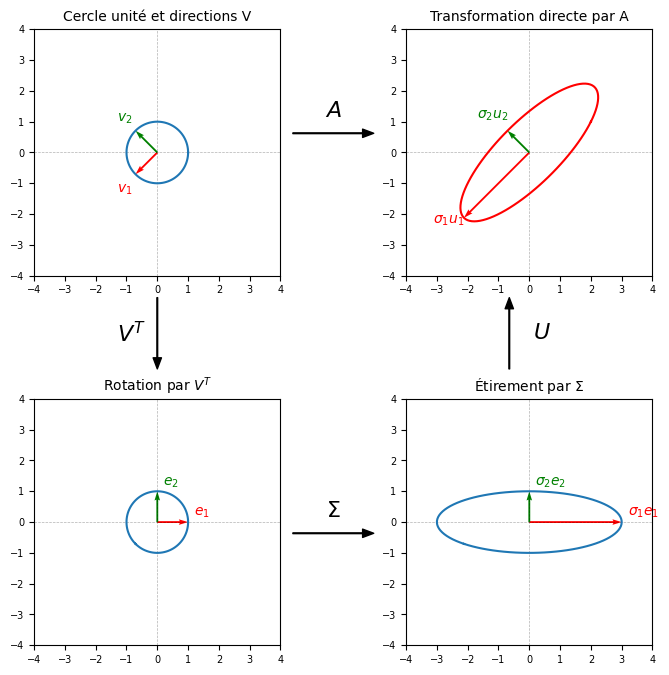
\includegraphics[width=1\textwidth]{geometriedesvd.png}
    \caption{Illustration géométrique de la DVS générée via Python.}
    \label{fig:svd_python}
\end{figure}
\clearpage
\subsection*{Le Premier Vecteur Singulier $v_1$ }

\noindent Nous avons défini les vecteurs singuliers à droite $v_i$ comme étant les vecteurs propres de la matrice $A^{\top} A$. Nous comprendrons ces vecteurs singuliers {un par un, de manière séquentielle}, au lieu de les considérer tous en même temps. Commençons par le premier vecteur singulier $v_1$ et sa valeur singulière associée $\sigma_1$.

\noindent Cette approche consiste à chercher la direction dans laquelle la matrice $A$ étire le plus les vecteurs. Cela revient à maximiser le ratio suivant :

\begin{equation}
    \max_{x \neq 0} \frac{\|Ax\|}{\|x\|} = \sigma_1
\end{equation}

\subsection*{Le Quotient de Rayleigh}
\addcontentsline{toc}{subsection}{Le Quotient de Rayleigh}

\noindent Jusqu'à présent, nous avons défini la DVS en supposant l'existence de la décomposition. Supposons que nous ne connaissons ni $U$, ni $\Sigma$, ni $V$.
Nous cherchons à maximiser le ratio $\frac{\|Ax\|}{\|x\|}$. Pour trouver un maximum, la méthode standard consiste à calculer la dérivée de la fonction et à l'égaler à zéro. Comme la norme euclidienne contient une racine carrée, les calculs deviennent plus compliqués. Pour simplifier, on maximise le carré de la fonction (qui a le même maximum), ce qui nous conduit au {Quotient de Rayleigh} :
\begin{equation}
    \max_{x \neq 0} \frac{\|Ax\|^2}{\|x\|^2} = \max_{x \neq 0} \frac{(Ax)^{\top} (Ax)}{x^{\top} x} = \max_{x \neq 0} \frac{x^{\top} A^{\top} A x}{x_1^2 + x_2^2 + \dots + x_n^2} = \max_{x \neq 0} \frac{x^{\top} S x}{x^{\top} x}
\end{equation}
où $S = A^{\top} A$ est une matrice symétrique.

Pour trouver ce maximum, nous devons calculer les dérivées partielles par rapport à chaque composante $x_i$ et les égaler à zéro. Calculons d'abord les dérivées du dénominateur et du numérateur séparément :

$$\frac{\partial}{\partial x_i} (x^{\top} x) = \frac{\partial}{\partial x_i} (x_1^2 + \dots + x_n^2) = 2x_i$$

$$\frac{\partial}{\partial x_i} (x^{\top} S x) = \frac{\partial}{\partial x_i} \left( \sum_i \sum_j S_{ij} x_i x_j \right) = 2 \sum_j S_{ij} x_j = 2(Sx)_i$$

\noindent Pour trouver ce maximum, nous devons calculer les dérivées partielles par rapport à chaque composante $x_i$ et les égaliser à zéro. Calculons d'abord les dérivées du dénominateur et du numérateur séparément :

$$\frac{\partial}{\partial x_i} (x^{\top} x) = \frac{\partial}{\partial x_i} (x_1^2 + \dots + x_n^2) = 2x_i$$

$$\frac{\partial}{\partial x_i} (x^{\top} S x) = \frac{\partial}{\partial x_i} \left( \sum_i \sum_j S_{ij} x_i x_j \right) = 2 \sum_j S_{ij} x_j = 2(Sx)_i$$

\noindent Ensuite, nous appliquons la règle de dérivation d'un quotient ($\frac{f'g - fg'}{g^2} = 0 \implies f'g - fg' = 0$). Pour que la dérivée globale soit nulle, le numérateur de cette dérivée doit obligatoirement s'annuler. Cela nous donne l'équation suivante :

$$x^{\top} x \cdot (2Sx) - (x^{\top} Sx) \cdot 2x = 0$$

\noindent Nous pouvons maintenant simplifier cette équation. En divisant chaque terme par $2$ et en réorganisant, nous obtenons :

$$(x^{\top} x) Sx = (x^{\top} Sx) x$$

\noindent Divisons ensuite les deux côtés par $(x^{\top} x)$ :

$$\frac{(x^{\top} x) Sx}{x^{\top} x} = \frac{(x^{\top} Sx) x}{x^{\top} x}$$

\noindent  Ce qui se simplifie pour donner notre résultat final :

$$Sx = \left( \frac{x^{\top} Sx}{x^{\top} x} \right) x$$

\noindent Elle correspond exactement à la définition d'une équation aux valeurs propres ($Sx = \lambda x$). Par conséquent :
\begin{itemize}
    \item Le vecteur $x$ qui maximise notre ratio est par définition un {vecteur propre} de $S$ (notre premier vecteur singulier $v_1$).
    \item Le terme entre grandes parenthèses, qui représente notre maximum, est la {valeur propre} $\lambda$ correspondante (qui est égale à $\sigma_1^2$).
\end{itemize}

\begin{example}
    \noindent Dans l'Exemple 8, nous avions effectué la décomposition en valeurs singulières de la matrice $A$, et nous avions trouvé le premier vecteur singulier $v_1$ ainsi que la valeur singulière maximale $\sigma_1 = \sqrt{6}$. Appliquons maintenant le Quotient de Rayleigh.
\end{example}

\noindent Rappelons notre matrice symétrique $S = A^{\top} A$ de l'exemple 8  :
$$S = \begin{bmatrix} 5 & -2 & 1 \\ -2 & 1 & 0 \\ 1 & 0 & 1 \end{bmatrix}$$

\noindent Nous voulons montrer que le quotient de Rayleigh atteint sa valeur maximale dans la direction du premier vecteur singulier $v_1$. Pour faciliter les calculs, il n'est pas nécessaire de rendre le vecteur unitaire ; en effet, dans le quotient de Rayleigh, la longueur du vecteur n'a pas d'importance, seule sa direction compte. C'est pourquoi nous utilisons directement notre vecteur non normalisé :

Étape 1 : Calcul du dénominateur (la norme au carré du vecteur) :
$$x^{\top} x = 5^2 + (-2)^2 + 1^2 = 25 + 4 + 1 = 30$$

Étape 2 : Calcul du produit matrice-vecteur $Sx$ :
$$Sx = \begin{bmatrix} 5 & -2 & 1 \\ -2 & 1 & 0 \\ 1 & 0 & 1 \end{bmatrix} \begin{bmatrix} 5 \\ -2 \\ 1 \end{bmatrix} = \begin{bmatrix} (25 + 4 + 1) \\ (-10 - 2 + 0) \\ (5 + 0 + 1) \end{bmatrix} = \begin{bmatrix} 30 \\ -12 \\ 6 \end{bmatrix}$$

Étape 3 : Calcul du numérateur $x^{\top} S x$ :
$$x^{\top} S x = \begin{bmatrix} 5 & -2 & 1 \end{bmatrix} \begin{bmatrix} 30 \\ -12 \\ 6 \end{bmatrix} = (5 \times 30) + (-2 \times -12) + (1 \times 6) = 150 + 24 + 6 = 180$$

Étape 4 : Quotient de Rayleigh :
$$\frac{x^{\top} S x}{x^{\top} x} = \frac{180}{30} = 6$$

\noindent Le résultat de ce quotient est très exactement $6$. Cela correspond à notre plus grande valeur propre $\lambda_1 = 6$, ce qui confirme que $\lambda_1 = \sigma_1^2 = (\sqrt{6})^2 = 6$. Nous avons ainsi vérifie numériquement que le quotient de Rayleigh trouve la variance maximale exactement dans la direction du premier vecteur singulier $v_1$.

\begin{definition}[Norme Spectrale d'une Matrice]
    Pour tout vecteur $x \in \mathbb{R}^n \setminus \{0\}$, la norme spectrale d'une matrice $A \in \mathbb{R}^{m \times n}$ est définie par :

    \begin{equation}
        \|A\|_2 := \max_{x \neq 0} \frac{\|Ax\|_2}{\|x\|_2}
    \end{equation}
\end{definition}

\begin{definition}[Norme de Frobenius]
    Pour une matrice $A \in \R^{m \times n}$ de rang $r$, elle est définie par la racine carrée de la somme des carrés de ses valeurs singulières :

    \begin{equation}
        \|A\|_F = \sqrt{\sigma_1^2 + \sigma_2^2 + \dots + \sigma_r^2} = \sqrt{\sum_{i=1}^{r} \sigma_i^2}
    \end{equation}
\end{definition}

\begin{theorem}
    La norme spectrale de $A$ est sa plus grande valeur singulière $\sigma_1$.
\end{theorem}

\begin{proof}
    D'après la définition de la norme spectrale :
    $$ \|A\|_2 = \max_{x \neq 0} \frac{\|Ax\|_2}{\|x\|_2}. $$

    \noindent Pour simplifier les calculs, nous en prenons le carré :
    $$ \|A\|_2^2 = \max_{x \neq 0} \frac{\|Ax\|_2^2}{\|x\|_2^2} = \max_{x \neq 0} \frac{x^{\top} A^{\top} A x}{x^{\top} x} = \max_{x \neq 0} R(x), $$
    où $R(x)$ est le quotient de Rayleigh pour la matrice $S = A^{\top} A$.

    \noindent Le maximum du quotient de Rayleigh est atteint dans la direction du vecteur propre correspondant à la plus grande valeur propre $\lambda_1$ de $S$. Par conséquent :
    $$ \|A\|_2^2 = \lambda_1. $$

    \noindent D'après la DVS, les valeurs propres de $S$ sont les carrés des valeurs singulières de $A$ : $\lambda_1 = \sigma_1^2$. En conclusion :
    $$ \|A\|_2 = \sigma_1. $$
\end{proof}
\clearpage

\subsection*{Approximation Matricielle}
\addcontentsline{toc}{subsection}{Approximation Matricielle}
La Décomposition en Valeurs Singulières permet d'exprimer toute matrice $A$ comme une somme de matrices de rang 1, chacune étant pondérée par sa propre valeur singulière ($\sigma_i$). L'ordre décroissant des valeurs singulières détermine directement le niveau de dominance de ces composantes sur la matrice.

Grâce à cette structure, il est possible d'approximer efficacement la matrice $A$ en ne conservant qu'un nombre limité de termes (les $k$ premiers) de cette somme. Cette approche nous conduit naturellement au concept fondamental d'approximation matricielle de rang faible (\textit{low-rank approximation}), qui permet de préserver la grande majorité de l'information structurelle de la matrice d'origine.

Pour une matrice $A$ de ${rang}(A) = r$, l'approximation de rang $k$ (où $k < r$) est définie par l'expression suivante :

\begin{equation}
    \widehat{A}(k) = \sum_{i=1}^{k} \sigma_i u_i v_i^{\top}
\end{equation}

\begin{theorem}[Eckart–Young Théorème - Norme Spectral]
    Soit $A \in \R^{m \times n}$ une matrice de rang $r$, et soit $B \in \R^{m \times n}$ une matrice de rang $k$, l'inégalité suivante est toujours satisfaite :
    \begin{equation}
        \|A - B\|_2 \geq \|A - A_k\|_2 = \sigma_{k+1}
    \end{equation}
    Ce théorème affirme que la matrice $A_k$, obtenue par la DVS, est la meilleure approximation de rang $k$ de la matrice $A$ au sens de la norme spectrale.
\end{theorem}

\begin{proof}
    Supposons par l'absurde qu'il existe une matrice $B$ de rang $k$ telle que :
    \begin{equation}
        \|A - B\|_2 < \|A - A_k\|_2 = \sigma_{k+1}
    \end{equation}
    Pour tout vecteur non nul $w \in \R^n$, nous aurions $\|(A - B)w\|_2 < \sigma_{k+1}\|w\|_2$. En particulier, pour tout $w \in \ker(B)$ (où $Bw = 0$), cela impliquerait :
    \begin{equation} \label{eq:1}
        \|Aw\|_2 < \sigma_{k+1}\|w\|_2
    \end{equation}


    \noindent D'autre part, considérons le sous-espace $V_{k+1} = \text{span}\{v_1, \dots, v_{k+1}\}$. Pour tout $w \in V_{k+1}$, $w$ peut s'écrire comme $w = \sum_{i=1}^{k+1} c_i v_i$. Par l'orthogonalité des vecteurs $v_i$ et puisque $\sigma_1 \ge \dots \ge \sigma_{k+1}$, nous avons :
    \begin{equation} \label{eq:2}
        \|Aw\|_2 = \left\| \sum_{i=1}^{k+1} c_i \sigma_i u_i \right\|_2 = \sqrt{\sum_{i=1}^{k+1} c_i^2 \sigma_i^2} \ge \sigma_{k+1} \sqrt{\sum_{i=1}^{k+1} c_i^2} = \sigma_{k+1}\|w\|_2
    \end{equation}


    \noindent D'après le théorème du rang, $\dim(\ker(B)) = n - k$ et nous savons que $\dim(V_{k+1}) = k + 1$. La somme de leurs dimensions étant $(n-k) + (k+1) = n+1 > n$, il existe nécessairement un vecteur $w \neq 0$ tel que $w \in \ker(B) \cap V_{k+1}$.


    \noindent Cependant, pour ce vecteur $w$, les inégalités \eqref{eq:1} et \eqref{eq:2} sont contradictoires. Cette contradiction prouve qu'aucune matrice $B$ de rang $k$ ne peut surpasser l'approximation $A_k$.
\end{proof}

\begin{theorem} [Eckart–Young Théorème - Norme de Frobenius] Soit $A \in \mathbf{R}^{m \times n}$ une matrice de rang $r$, et soit $B \in \mathbf{R}^{m \times n}$ une matrice de rang $k$, l'inégalité suivante est toujours satisfaite :
    \begin{equation*}
        \|A - B\|_F^2 \geq \|A - A_k\|_F^2 = \sum_{i=k+1}^{r} \sigma_i^2
    \end{equation*}
    \noindent Ce théorème affirme que la matrice $A_k$, obtenue par la DVS, est la meilleure approximation de rang $k$ de la matrice $A$ au sens de la norme de Frobenius.
\end{theorem}

\noindent \textbf{Démonstration.}
Toute matrice $B \in \mathbf{R}^{m \times n}$ de rang $k$ peut s'écrire sous la forme d'une factorisation $k$ $B = CR$, où $C \in \mathbf{R}^{m \times k}$ et $R \in \mathbf{R}^{k \times n}$.

\noindent On peut toujours paramétrer une telle factorisation en introduisant une décomposition DVS de $B$ :
$B = U_B \Sigma_B V_B^{\top}$, et en posant
$C = U_B \Sigma_B$ et $R = V_B^{\top}$.
Dans cette écriture, on a bien $RR^{\top} = I_k$ et les colonnes de $C$ sont orthogonales, avec
$C^{\top}C = \Sigma_B^2$ diagonale.

\noindent En utilisant l'identité $\|X\|_F^2 = \text{tr}(X X^{\top})$, nous pouvons développer la fonction d'erreur $E = \|A - CR\|_F^2$ sous la forme suivante :
\begin{align}
    E & = \text{tr}\left( (CR - A)(CR - A)^{\top} \right) \nonumber                                                           \\
      & = \text{tr}(C R R^{\top} C^{\top}) - \text{tr}(C R A^{\top}) - \text{tr}(A R^{\top} C^{\top}) + \text{tr}(A A^{\top})
\end{align}

\noindent Afin d'analyser la structure des solutions de rang $k$, on considère les conditions stationnaires par rapport à $C$ et $R$.

\noindent \textbf {Remarque 1.}
\textit{Pour le calcul des dérivées matricielles impliquant l'opérateur de trace ($\text{tr}$), nous utilisons les identités standards suivantes :}
\begin{align*}
    \frac{\partial}{\partial X} \text{tr}(XA)         & = A^{\top}       \\
    \frac{\partial}{\partial X} \text{tr}(XAX^{\top}) & = XA^{\top} + XA \\
    \frac{\partial}{\partial X} \text{tr}(AX^{\top})  & = A
\end{align*}
\\

\noindent En dérivant par rapport à $C$, on obtient :
\begin{equation*}
    \frac{\partial E}{\partial C} = 2C R R^{\top} - 2A R^{\top}
\end{equation*}

\noindent De même, la dérivation par rapport à $R$ donne :
\begin{equation*}
    \frac{\partial E}{\partial R} = 2C^{\top}C R - 2C^{\top}A
\end{equation*}

\noindent Aux points stationnaires, on a donc :
\begin{equation*}
    C = A R^{\top}, \qquad C^{\top}A = (C^{\top}C)R
\end{equation*}

\noindent En combinant ces deux relations, on obtient :
\begin{equation*}
    (A^{\top}A)R^{\top} = R^{\top}(C^{\top}C)
\end{equation*}

\noindent Ce qui montre que les colonnes de $R^{\top}$ engendrent un sous-espace invariant de $A^{\top}A$, donc elles coïncident avec les vecteurs singuliers à droite associés aux $k$ plus grandes valeurs singulières, i.e. $R^{\top} = V_k^{\top}$.

\noindent Réciproquement, on obtient :
\begin{equation*}
    (AA^{\top})C = C(C^{\top}C)
\end{equation*}

\noindent Ce qui implique que les colonnes de $C$ appartiennent au sous-espace engendré par les vecteurs singuliers à gauche $U_k$ de $A$.
\clearpage
\noindent Ainsi, toute solution optimale de rang $k$ est de la forme :
\begin{equation}
    B = CR = U_k \Sigma_k V_k^{\top} = \sum_{i=1}^{k} \sigma_i u_i v_i^{\top}.
\end{equation}

\noindent L'erreur associée s'écrit alors :
\begin{equation}
    \|A - B\|_F^2 = \sum_{i \notin S} \sigma_i^2.
\end{equation}

\noindent Pour minimiser cette quantité, il est nécessaire de choisir les indices correspondant aux plus grandes valeurs singulières de $A$. Ainsi, on prend
\begin{equation}
    S = \{1, 2, \dots, k\},
\end{equation}

\noindent ce qui donne la meilleure approximation.

\noindent On obtient alors :
\begin{equation}
    \|A - B\|_F^2 = \sum_{i=k+1}^{r} \sigma_i^2, \quad \text{et} \quad B = A_k = U_k \Sigma_k V_k^{\top}.
\end{equation}

\noindent Cela conclut la démonstration du théorème d'Eckart–Young.
\hfill $\square$
\\
\\
\\
\\
\section*{Application de la DVS à la Compression d'Images}
\addcontentsline{toc}{section}{Application de la DVS à la compression d'images}
Dans cette section, nous mettons en évidence le lien direct entre l'approximation matricielle optimale et la compression de données à l'aide de la décomposition en valeurs singulières (DVS). Une image en niveaux de gris peut être modélisée mathématiquement par une matrice réelle $A \in \mathbf{R}^{n \times m}$, où $n$ et $m$ représentent respectivement le nombre de pixels verticaux et horizontaux. Grâce à la DVS, la matrice originale est décomposée selon ses composantes singulières sous la forme $A = U \Sigma V^{\top}$.

D'après le théorème d'Eckart–Young, la meilleure approximation de rang $k$ s'obtient en conservant uniquement les $k$ plus grandes valeurs singulières et leurs vecteurs singuliers associés. Sous les normes spectrale et de Frobenius, les valeurs singulières négligées ($\sigma_{k+1}, \dots, \sigma_r$) sont alors interprétées mathématiquement comme du bruit (\textit{noise}), ce qui permet de réaliser une réduction de dimension optimale tout en minimisant la perte d'information résiduelle.

Afin d'illustrer ce concept théorique en pratique, nous analysons deux images en niveaux de gris de dimensions $736 \times 414$ pixels, dont la matrice initiale est de rang égal à $414$. Nous appliquons la DVS pour reconstruire les matrices approximatives $A_k$ pour différentes valeurs de rang $k \in \{5, 10, 20, 50, 100\}$.

Enfin, nous procéderons à une analyse comparative des approximations obtenues pour ces deux images distinctes de mêmes dimensions, sous les mêmes valeurs de rang $k$.


\begin{figure}[H]
    \centering
    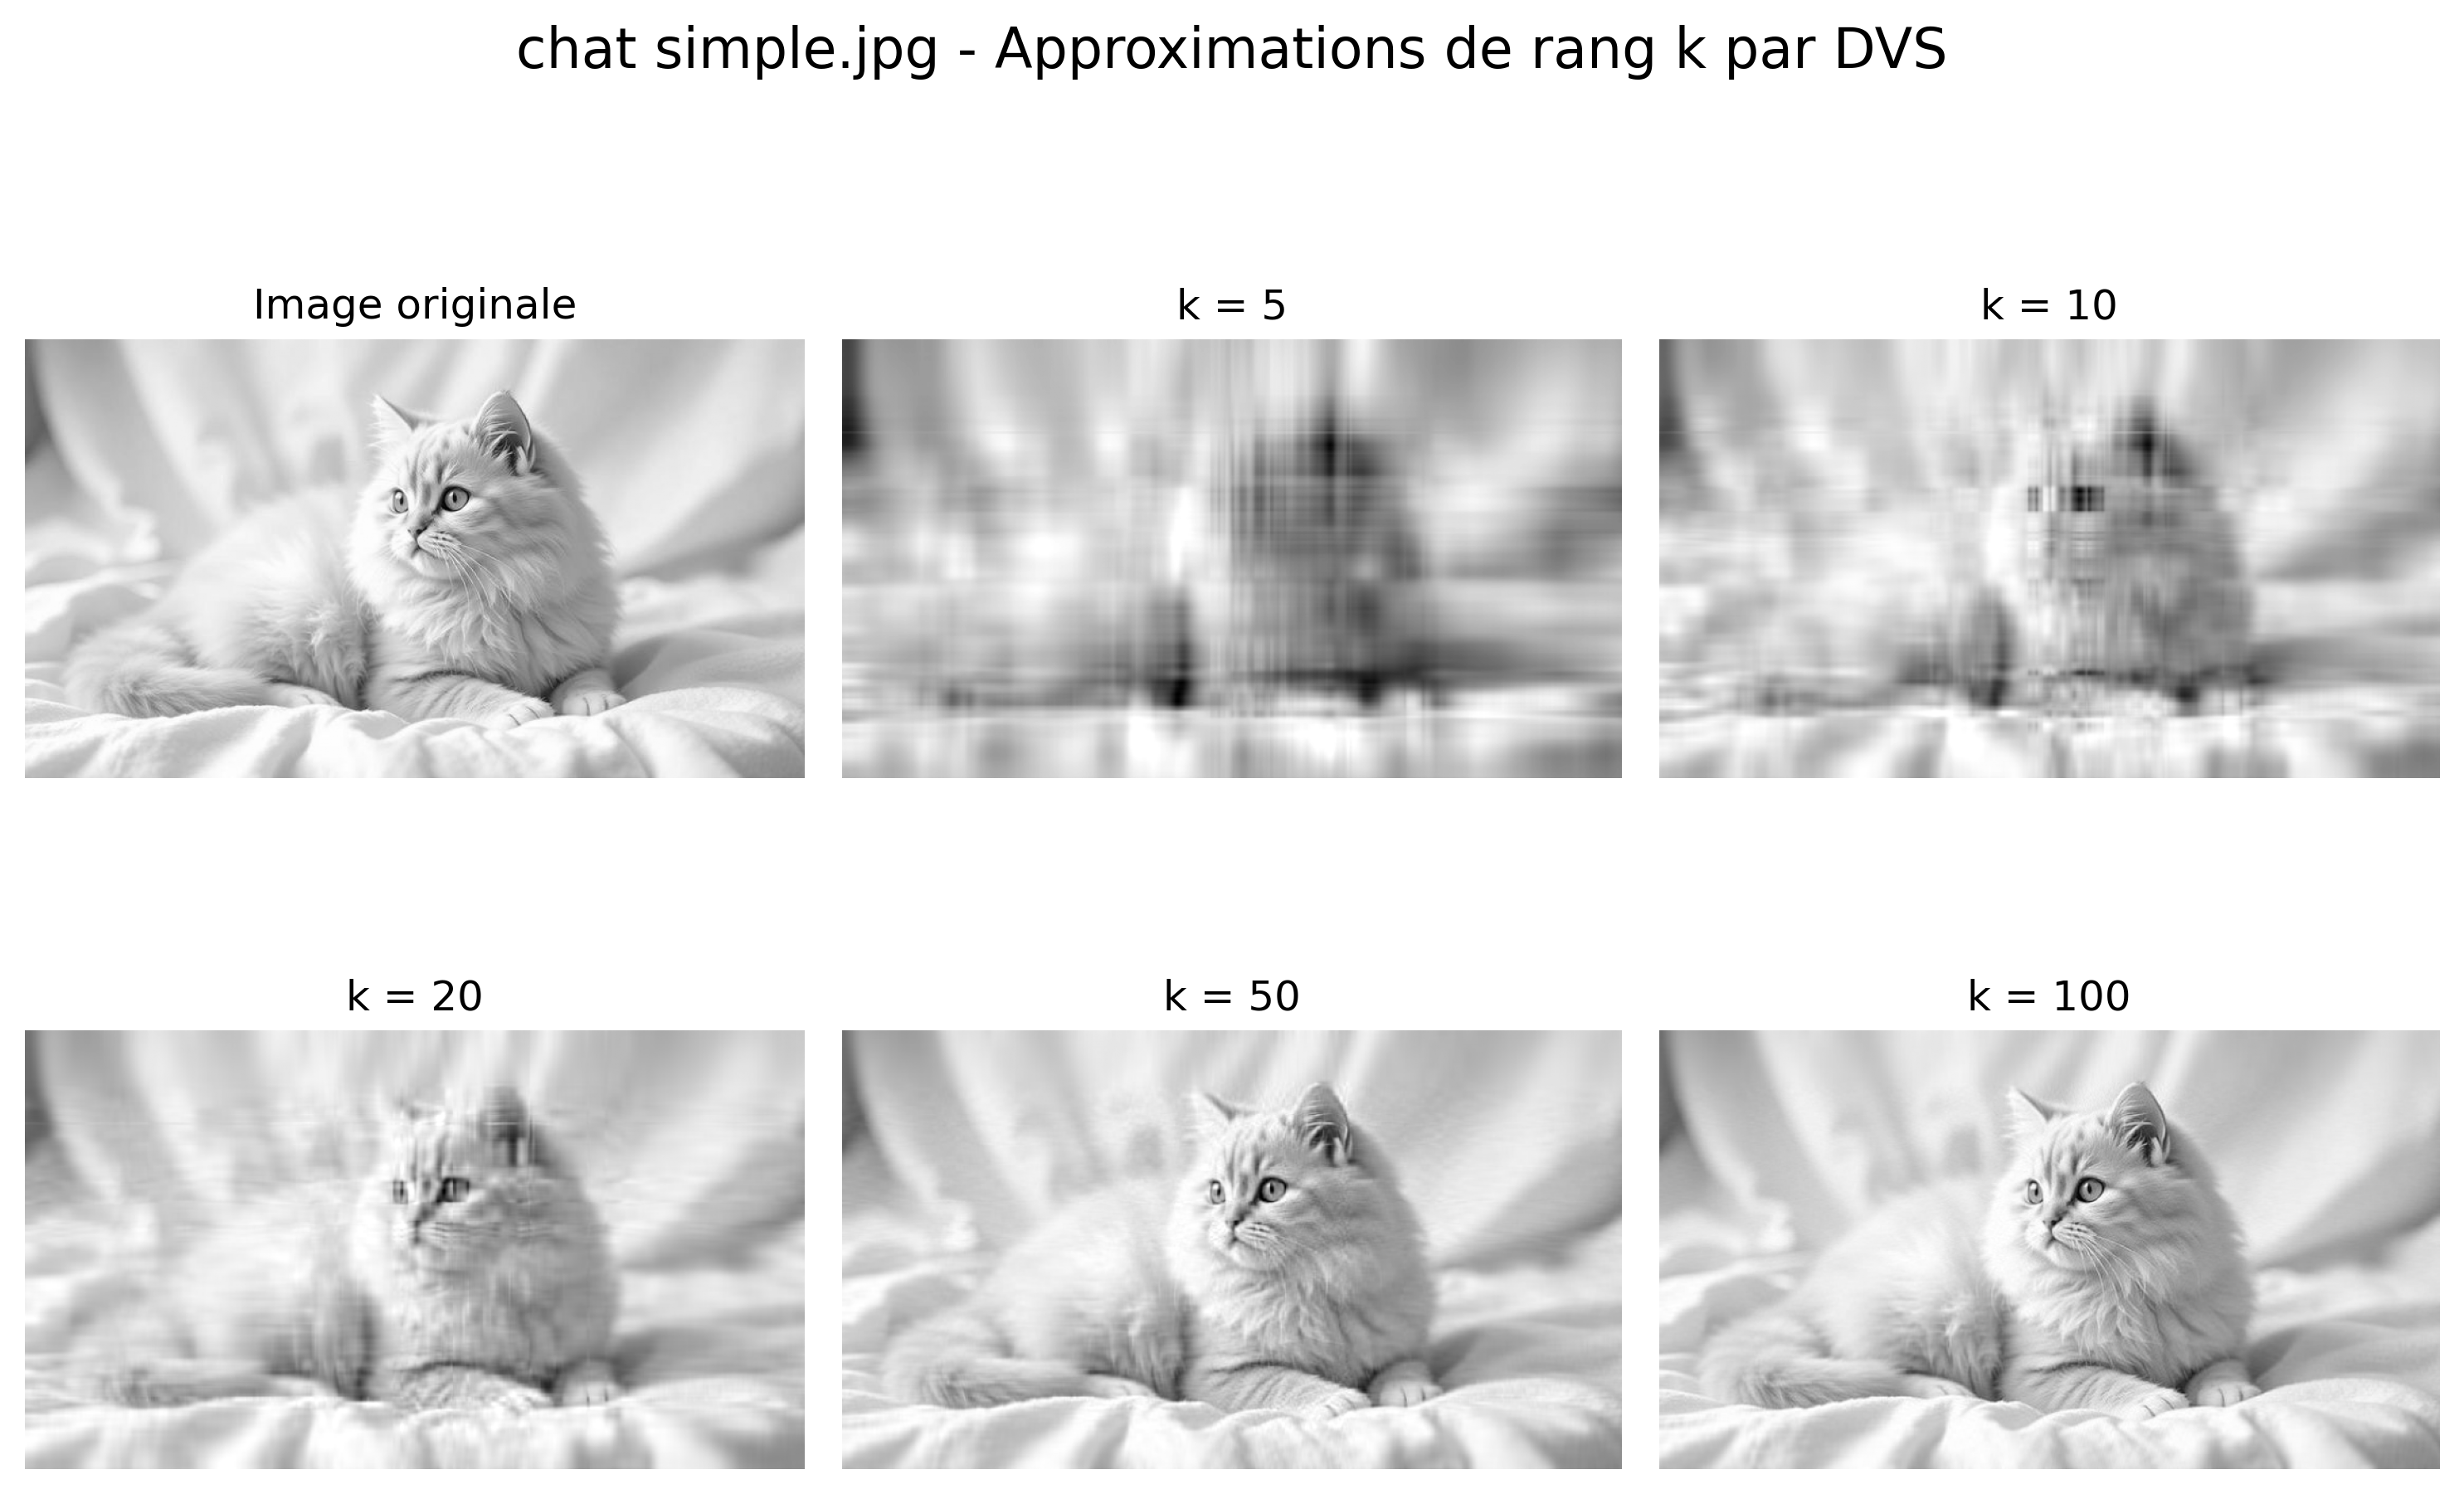
\includegraphics[width=0.9\textwidth]{chat_simple_svd_compression.png}
    \caption{}
    \label{fig:chat_simplemple_svd_compression}

    \vspace{0.5cm} % Ajoute un espace entre les images

    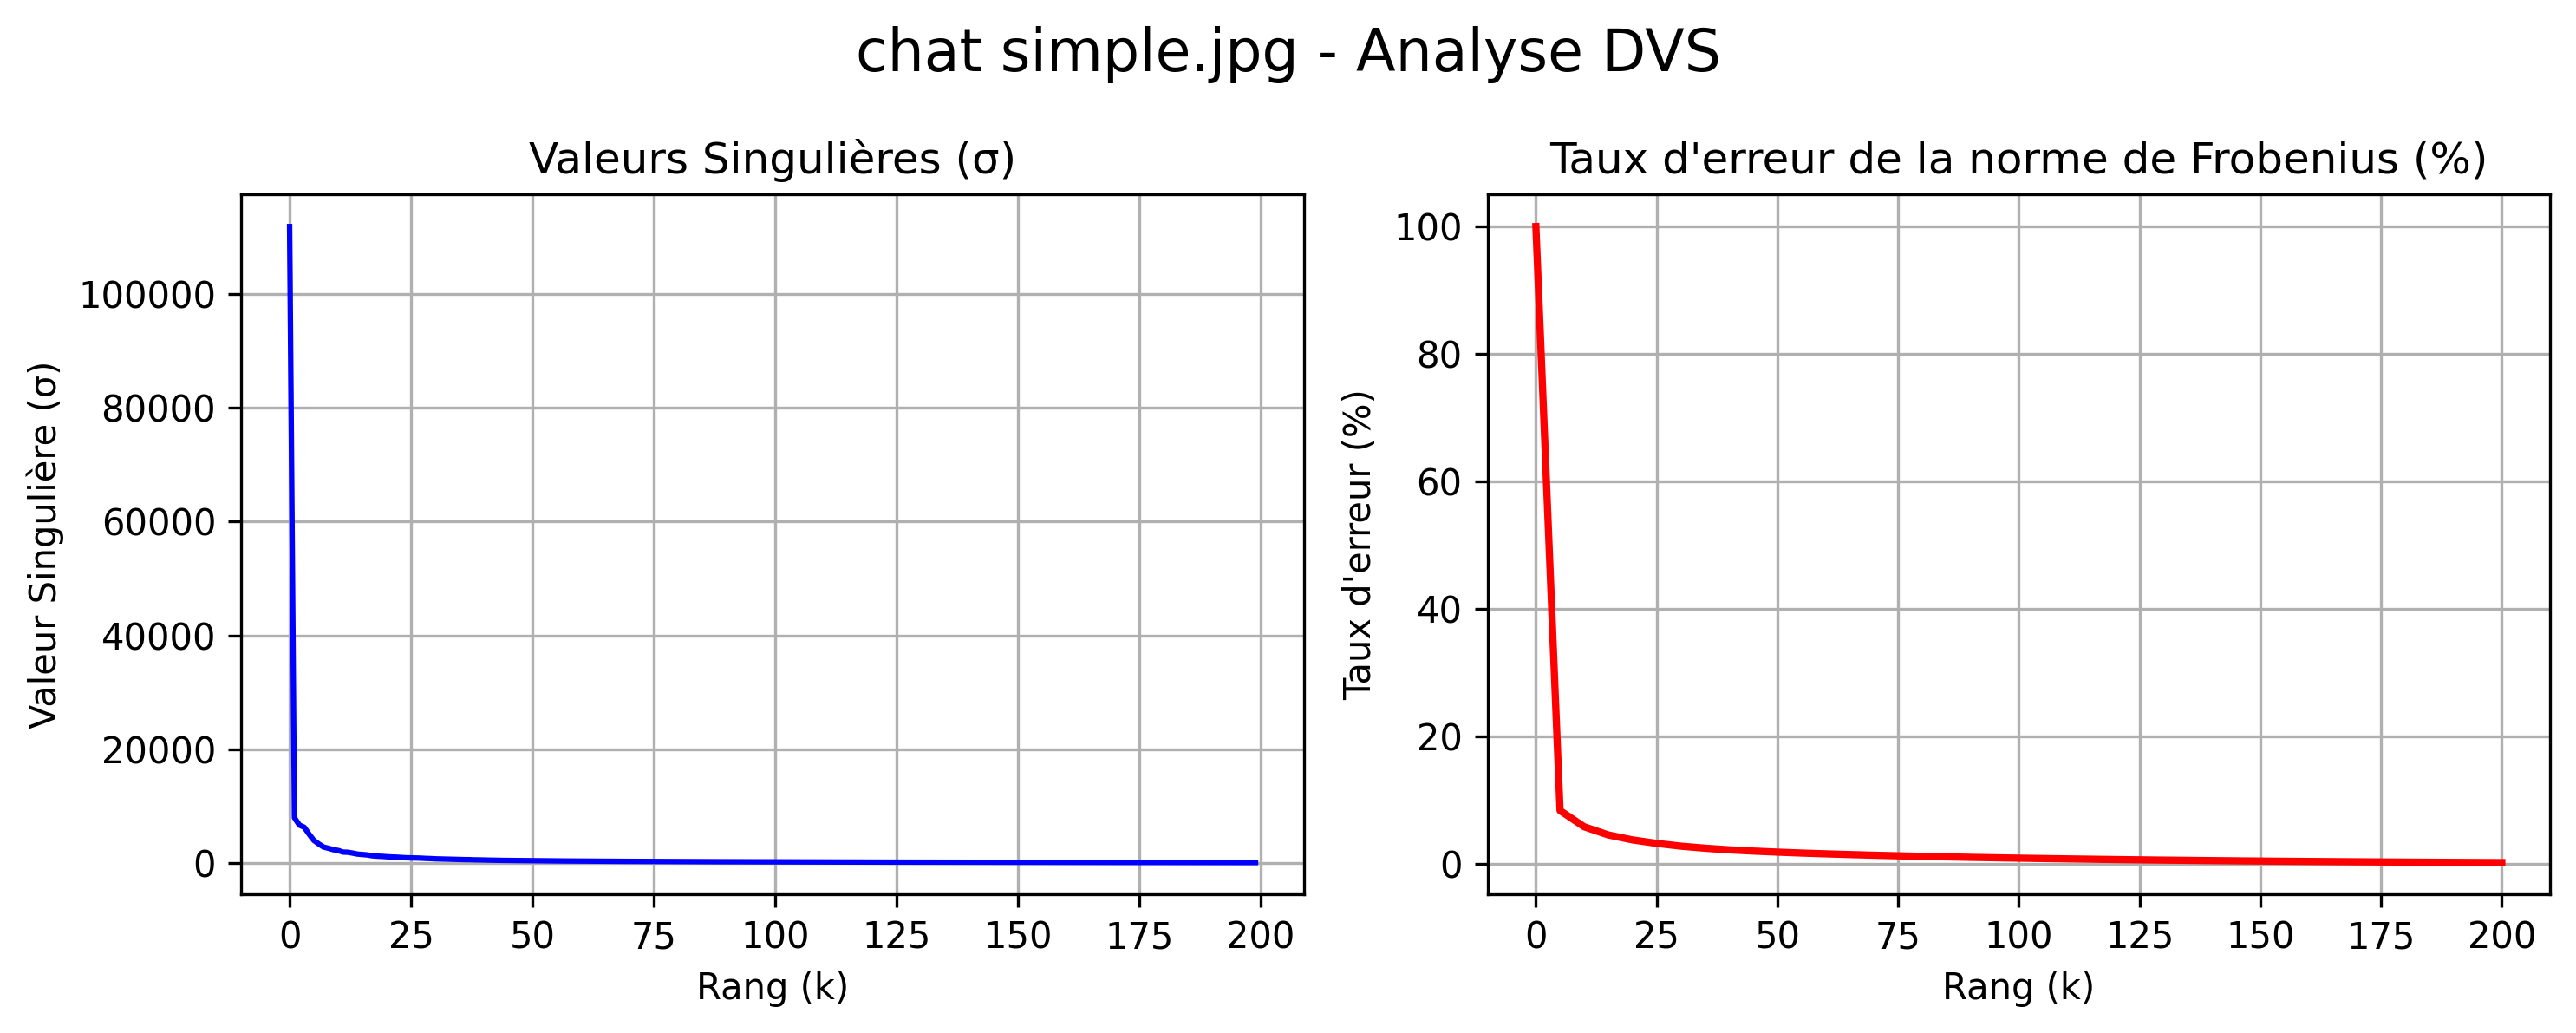
\includegraphics[width=0.9\textwidth]{chat_simple_svd_analysis_corrected.png}
    \caption{}
    \label{fig:chat_simplemple_svd_analysis}
\end{figure}
\noindent L'image montre un chat sur un arrière-plan doux (avec très peu de détails). En observant les différentes approximations de rang, l'évolution de la reconstruction est évidente :
\begin{itemize}
    \item Pour $k=5$ et $k=10$, l'image est floue et présente d'importants effets de blocs.
    \item À $k=20$, on distingue déjà très facilement la silhouette du chat.
    \item À $k=50$, on obtient une image très proche de l'originale.
    \item À $k=100$, la reconstruction est visuellement presque identique à l'image originale.
\end{itemize}

\vspace{0.3cm} % Paragraflar arası estetik bir boşluk

\noindent Sur le graphique des valeurs singulières, on observe une décroissance très rapide. Les toutes premières valeurs singulières sont largement dominantes, tandis que les suivantes diminuent drastiquement. Cela signifie que la plus grande partie de l'énergie (c'est-à-dire l'information essentielle de l'image) est concentrée dans ces premières valeurs singulières.

\vspace{0.3cm}

\noindent Le graphique de l'erreur relative suit exactement cette même tendance. Étant donné que les premières valeurs singulières contiennent l'essentiel de l'énergie de l'image et que les valeurs suivantes sont extrêmement petites, l'erreur tend très rapidement vers zéro à mesure que le rang $k$ augmente.
% --- Partie 2 : Analyse de c-1.jpg (Chat 1) ---
\begin{figure}[H]
    \centering
    % TODO: l'image chat_detaille_svd_compression.png est corrompue (fichier vide).
    % Pour la restaurer, relancez le script Python (Listing lst:svd_detail) avec
    % l'image source chat_detaille.jpg, puis décommentez la ligne ci-dessous.
    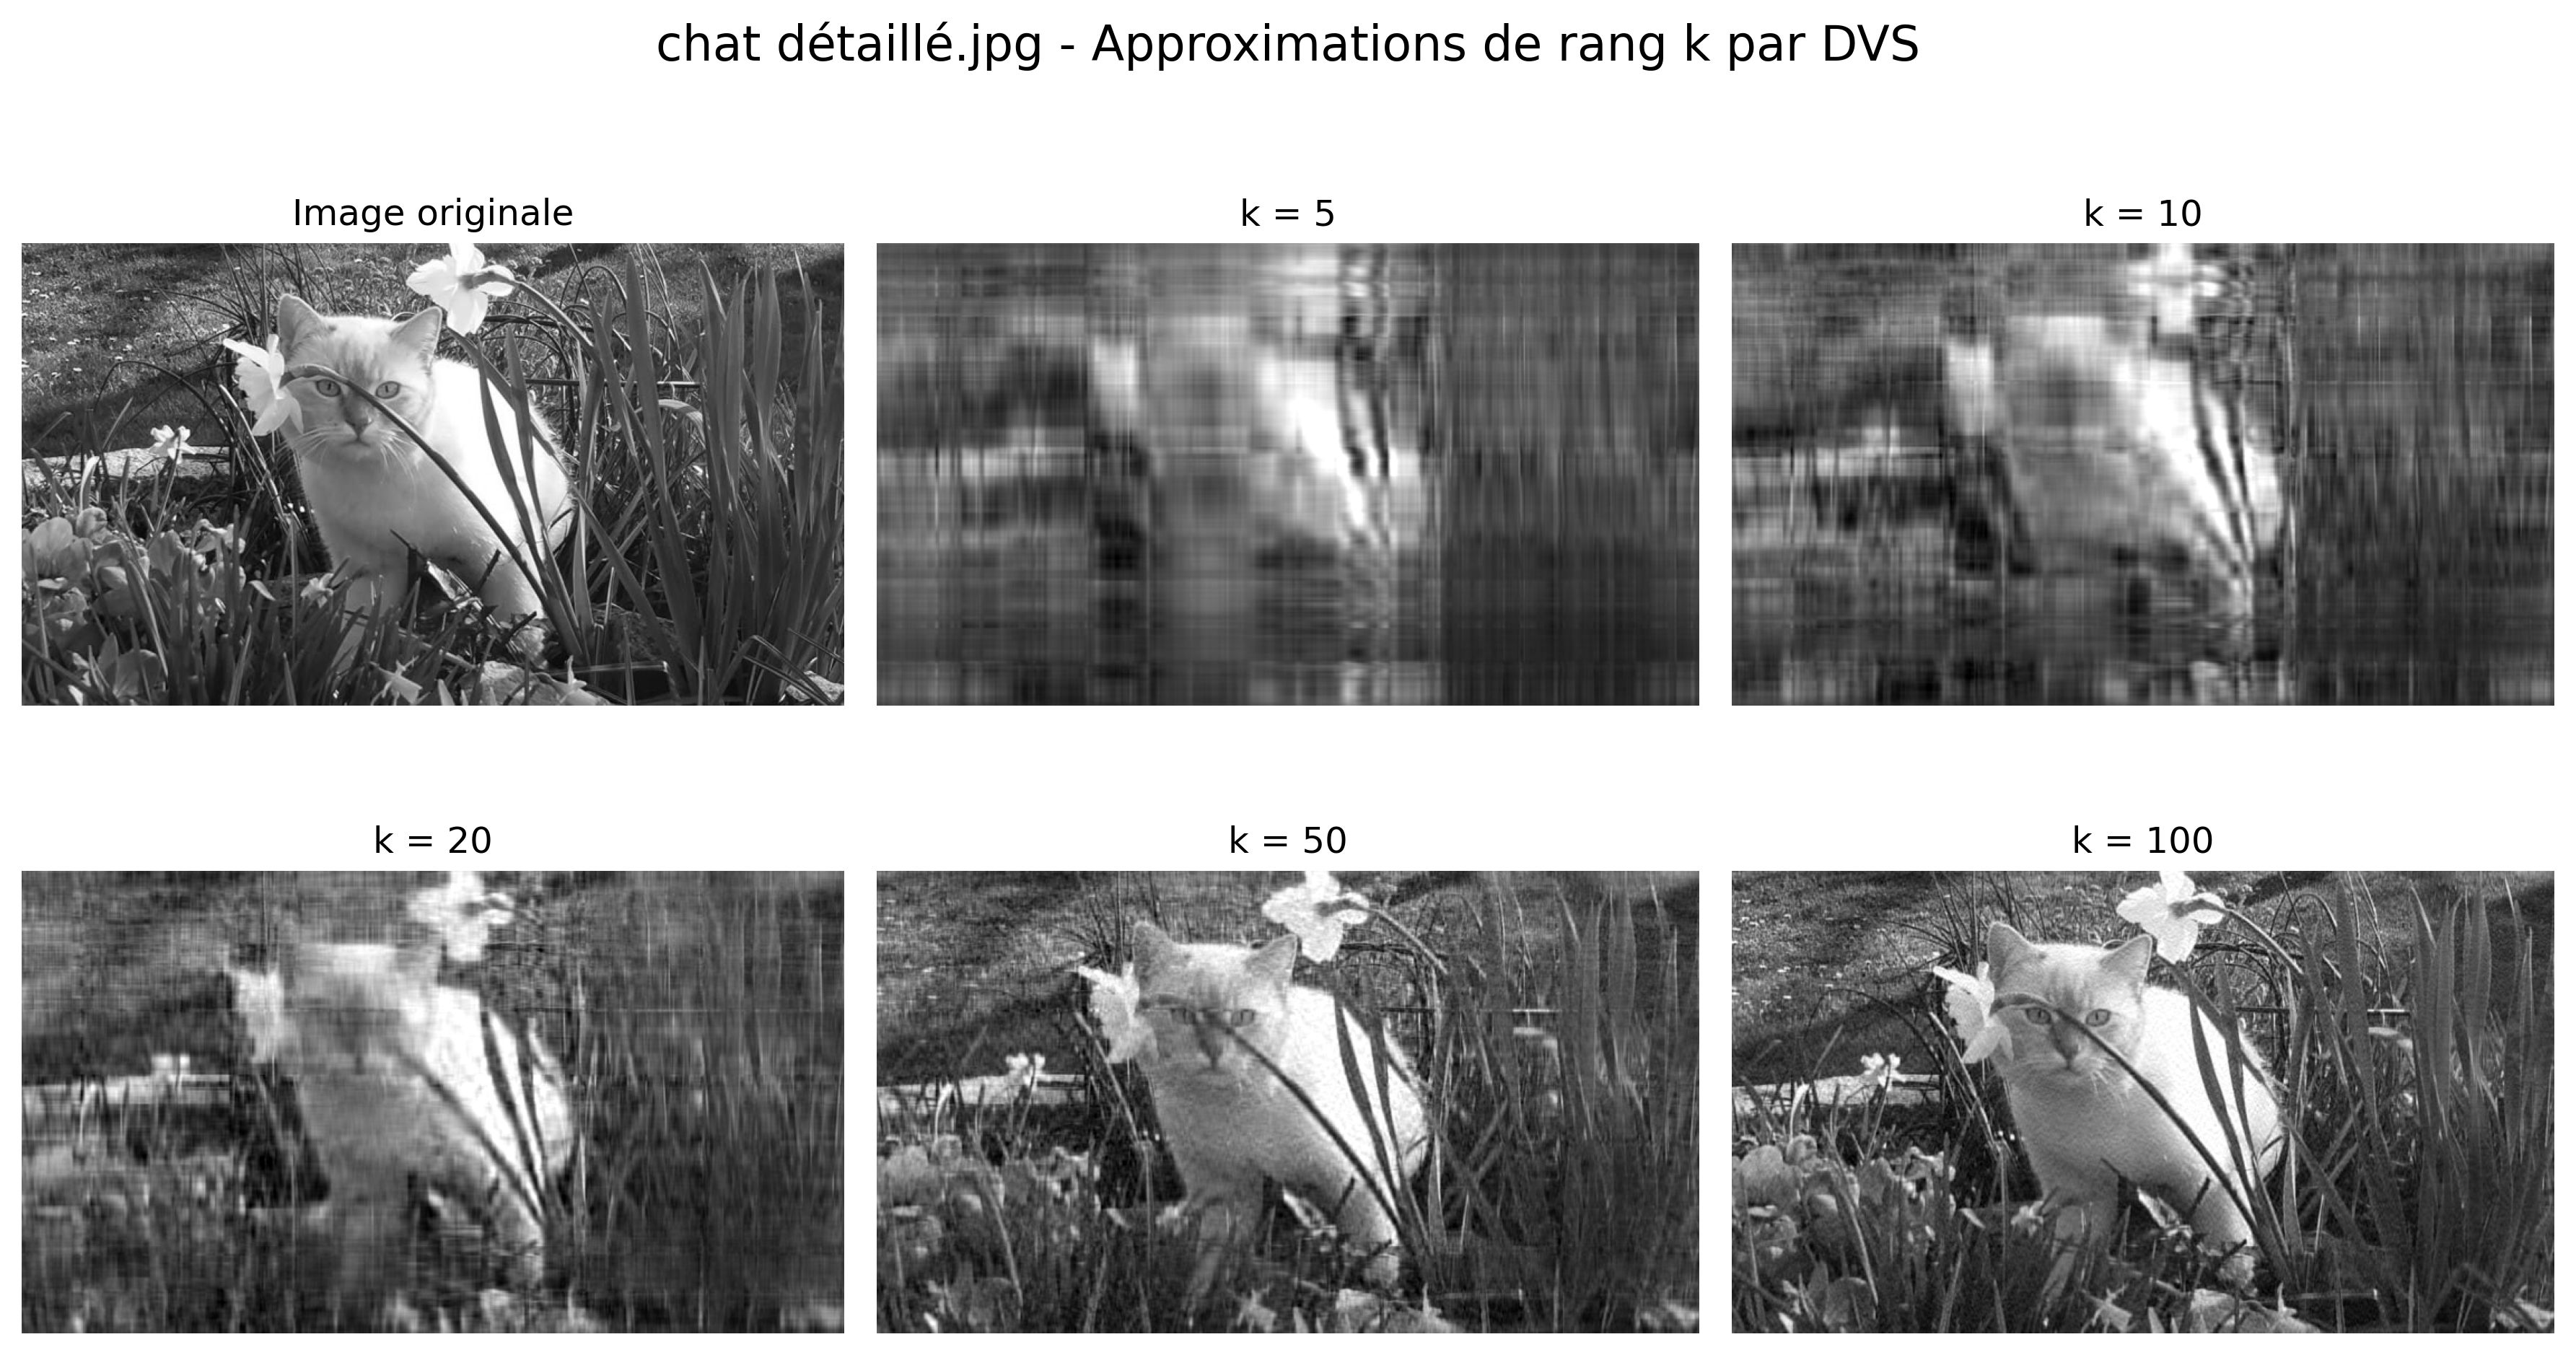
\includegraphics[width=0.9\textwidth]{chat_detaille_svd_compression.png}
    \caption{}
    \label{fig:chat_detaille_svd_compression}

    \vspace{0.5cm}

    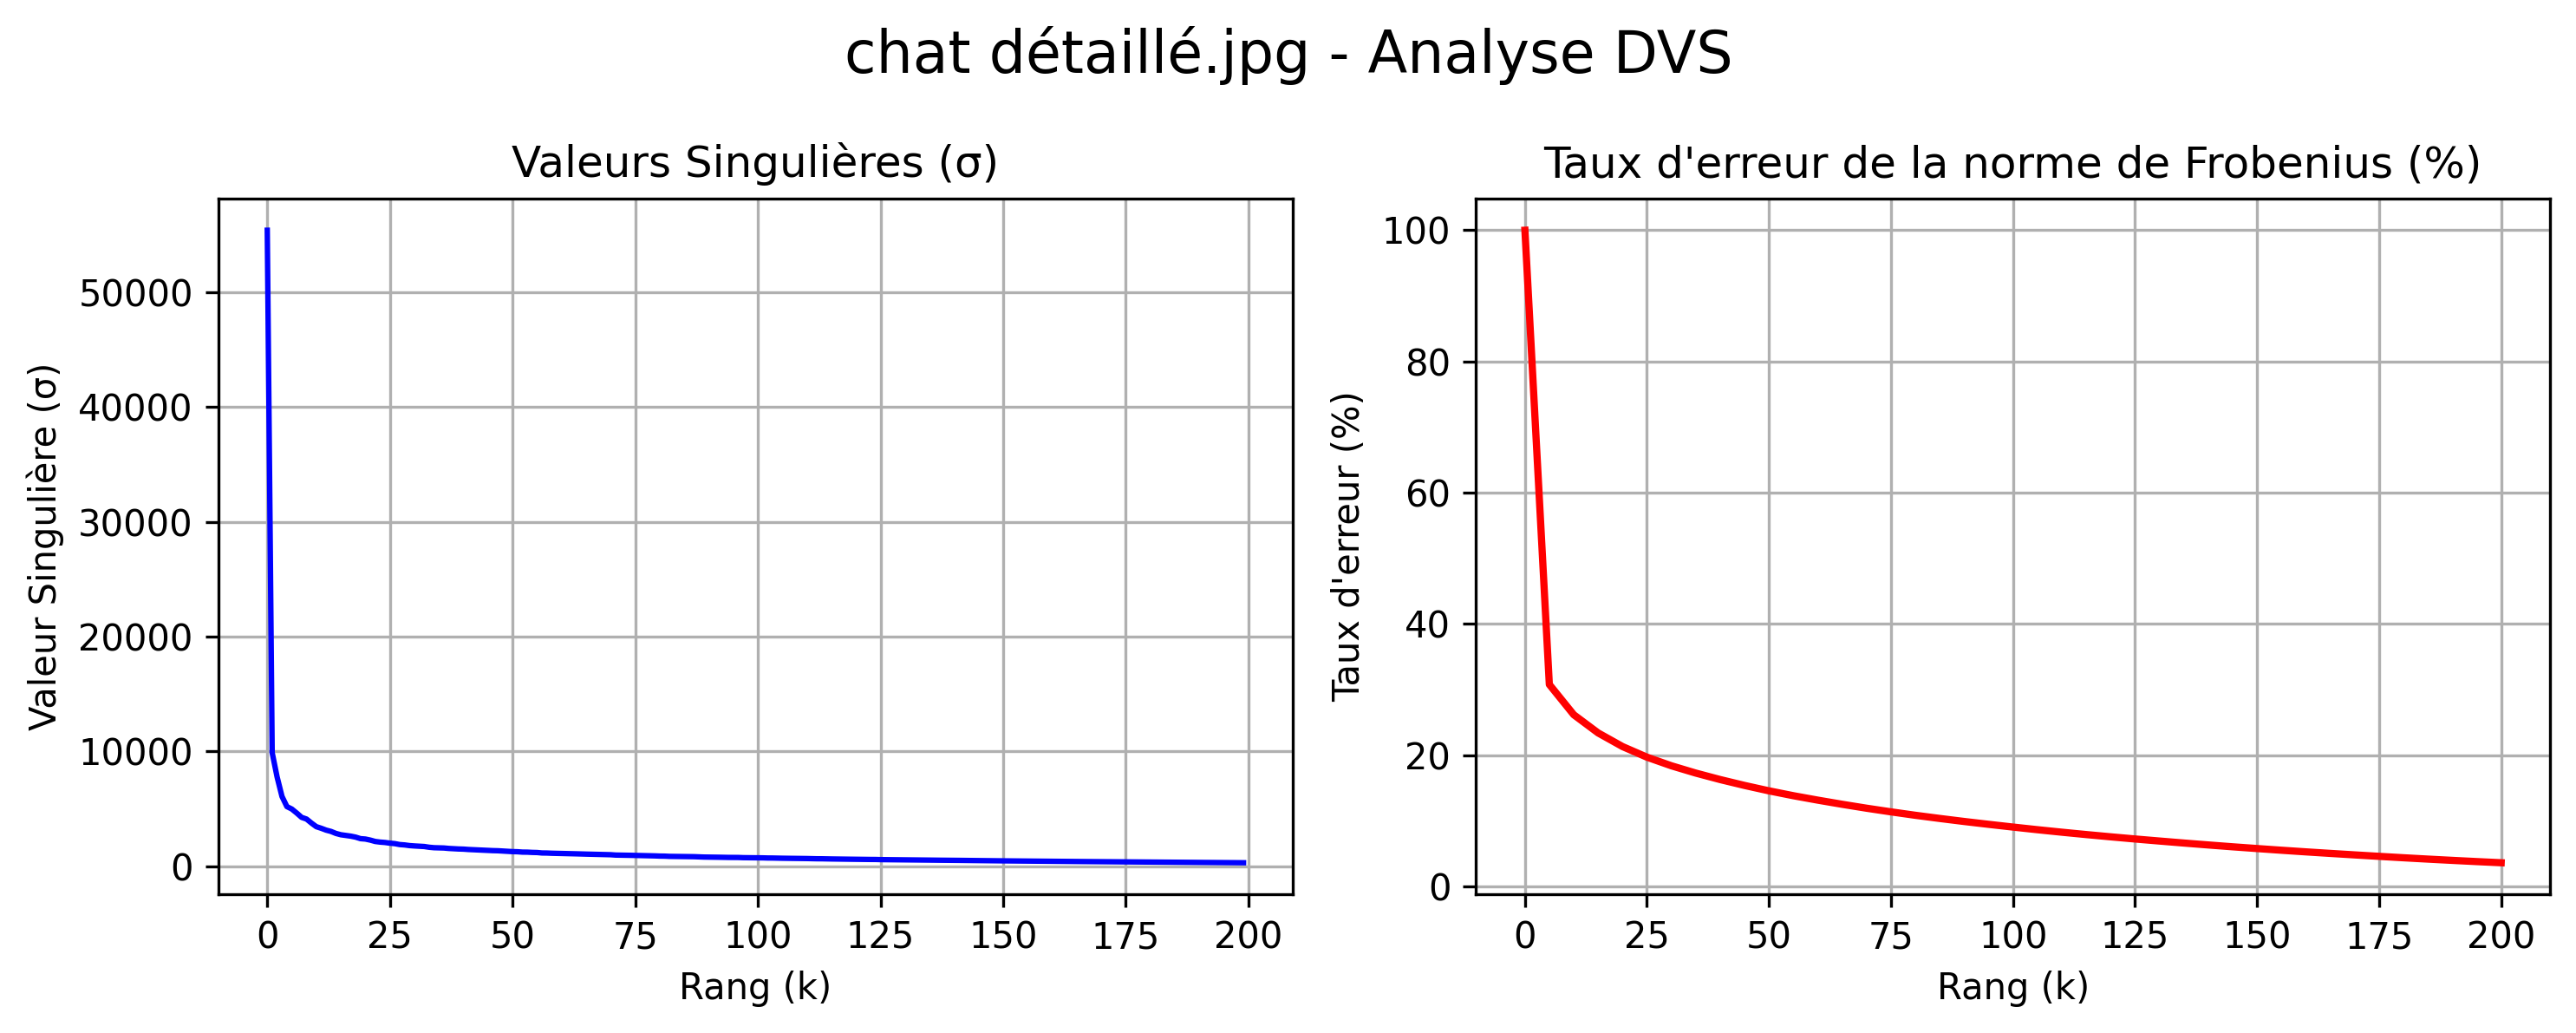
\includegraphics[width=0.9\textwidth]{chat_detaille_svd_analysis_corrected.png}
    \caption{}
    \label{fig:chat_detaille_svd_analysis}
\end{figure}
\noindent L'image montre un chat sur un arrière-plan complexe (végétation, texture dense). En observant les différentes approximations de rang, on constate que :
\begin{itemize}
    \item À $k=20$, on peut distinguer le chat et son environnement, mais la complexité des traits du visage du chat n'est pas encore résolue.
    \item À $k=50$, le rendu est un peu plus net. Cependant, comparé au chat précédent (qui possédait un arrière-plan doux), la plupart des détails fins restent indiscernables.
\end{itemize}
Autrement dit, pour cette image complexe, une poignée de valeurs singulières ne suffit absolument pas à la représenter fidèlement.

\vspace{0.3cm}

\noindent Sur le graphique de l'erreur relative en fonction du rang, on retrouve une courbe décroissante similaire. Toutefois, par rapport au premier chat, l'erreur est nettement plus élevée, en particulier dans l'intervalle de rang allant de $0$ à $25$. À titre d'exemple, pour la deuxième image, à $k \approx 25$, l'erreur est encore d'environ $20\%$, alors que pour la première image, au même rang $k$, elle est presque nulle.

\vspace{0.3cm}

\noindent Pour le premier chat, l'énergie est concentrée presque exclusivement dans les $20$ premières valeurs singulières. Tandis que pour le deuxième, il faut atteindre $k \approx 50$ ou plus pour obtenir la même fidélité. L'énergie mathématique est donc répartie sur un bien plus grand nombre de valeurs singulières.

% --- Partie 3 : Graphique comparatif PSNR et SSIM ---
\begin{figure}[H]
    \centering
    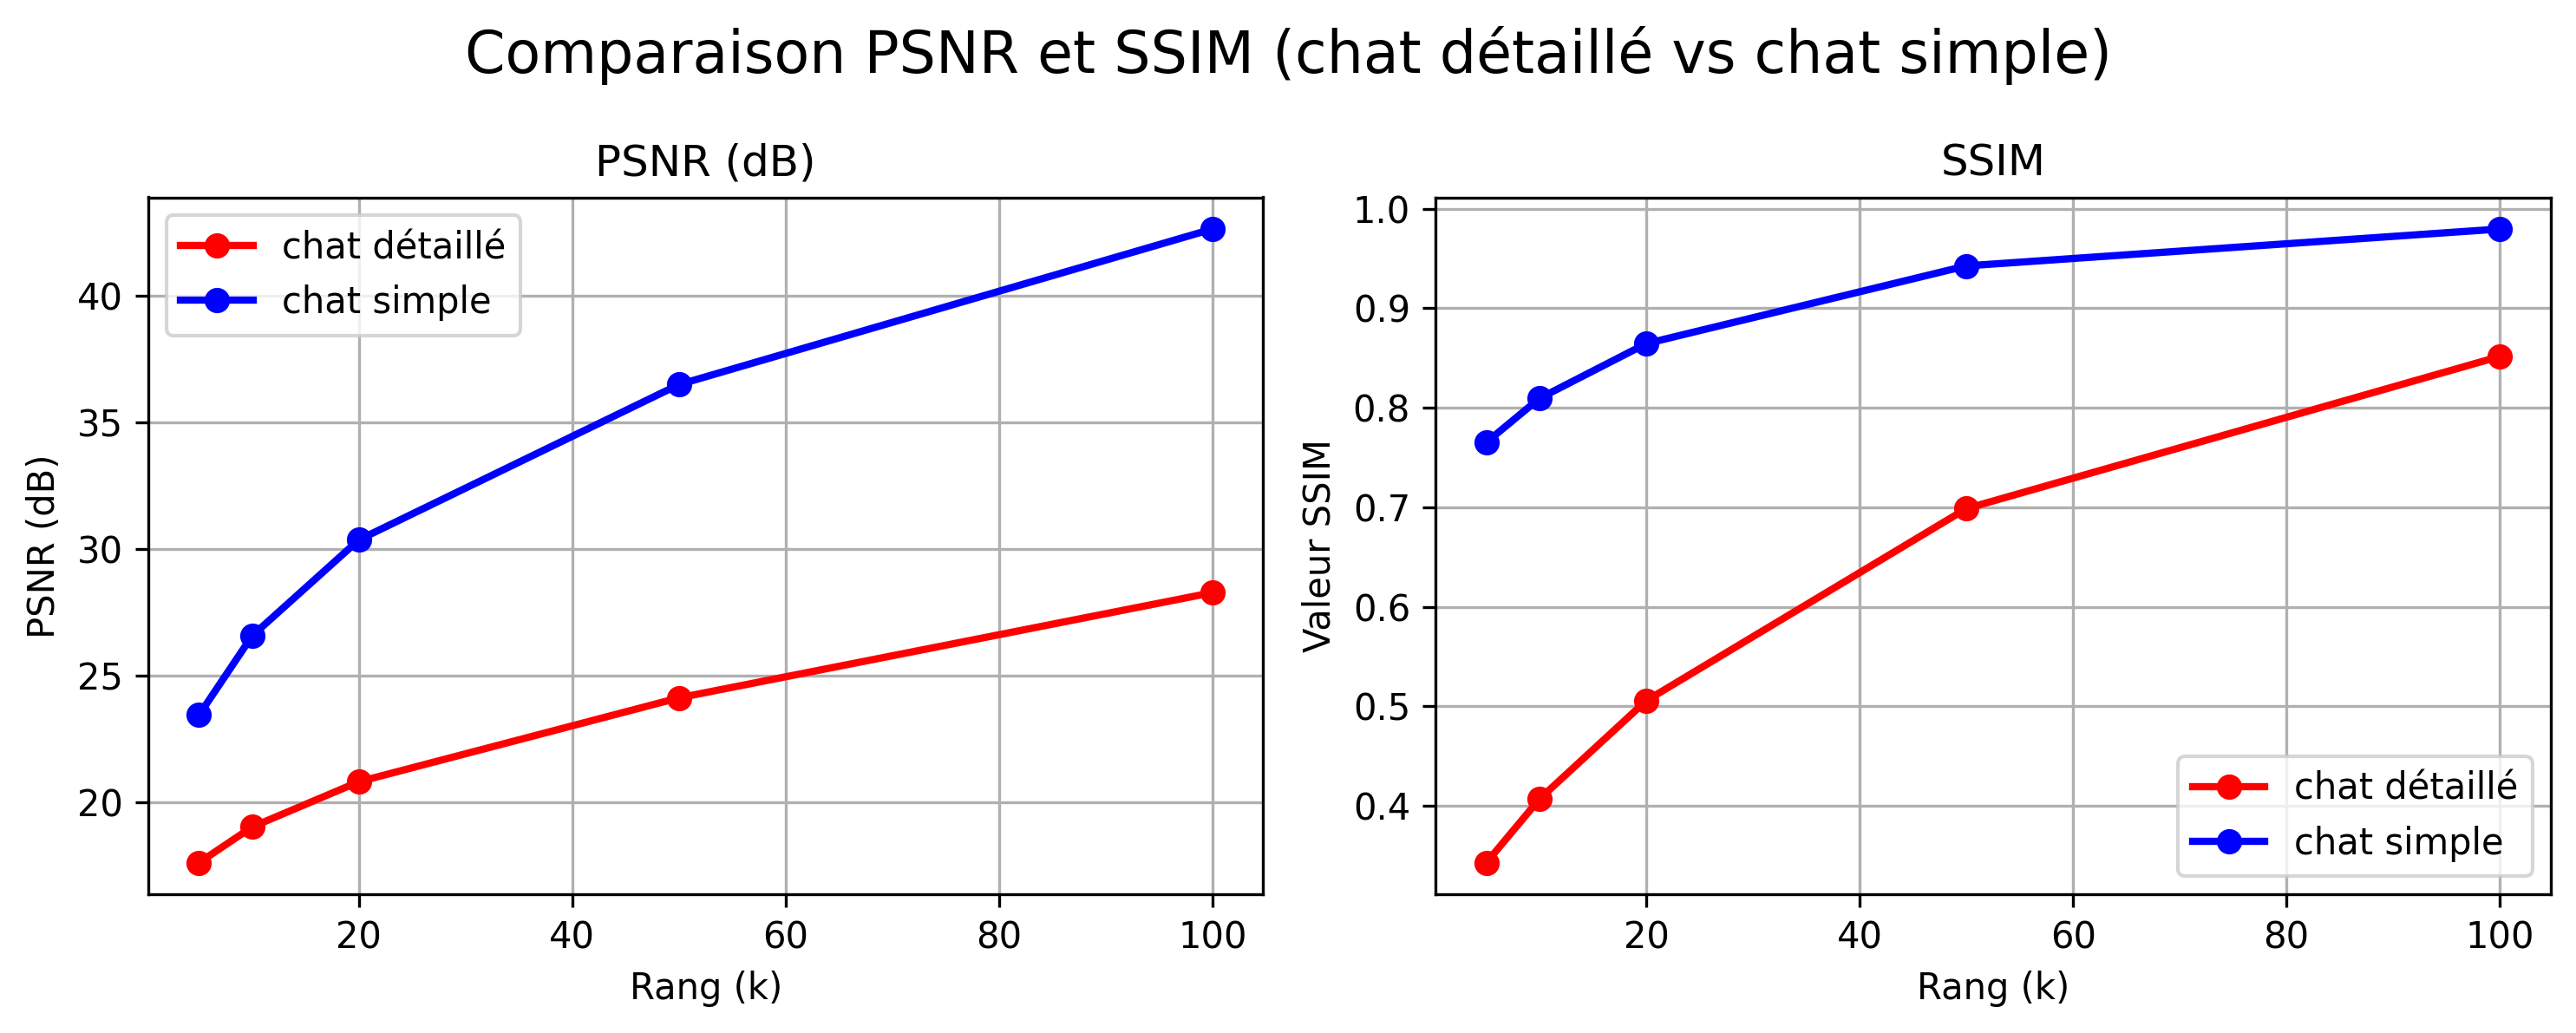
\includegraphics[width=0.9\textwidth]{psnr_ssim_comparison.png}
    \caption{}
    \label{fig:psnr_ssim_comparison}
\end{figure}

\vspace{0.3cm}

\noindent Le PSNR mesure à quel point l'image compressée ressemble à l'originale : plus il est élevé, meilleure est la qualité (son unité est le décibel, dB). Mathématiquement, pour une image en niveaux de gris où l'intensité maximale d'un pixel est de $255$, le PSNR est défini à partir de l'erreur quadratique moyenne (MSE - \textit{Mean Squared Error}) entre l'image originale $I$ et l'image reconstruite $K$, toutes deux de dimensions $m \times n$ :

\begin{equation}
    \text{MSE} = \frac{1}{mn} \sum_{i=1}^{m} \sum_{j=1}^{n} \left[ I(i,j) - K(i,j) \right]^2
\end{equation}

\begin{equation}
    \text{PSNR} = 10 \log_{10} \left( \frac{255^2}{\text{MSE}} \right) = 20 \log_{10} \left( \frac{255}{\sqrt{\text{MSE}}} \right)
\end{equation}
\begin{itemize}
    \item \textbf{$> 40$~dB :} Qualité presque sans perte (la différence n'est pas visible à l'œil nu).
    \item \textbf{Entre $30$ et $40$~dB :} Bonne qualité.
    \item \textbf{Entre $20$ et $30$~dB :} Qualité moyenne (la dégradation commence à se voir).
    \item \textbf{$< 20$~dB :} Faible qualité.
\end{itemize}

\noindent Sur le graphique, le PSNR augmente avec $k$ pour les deux images, mais la courbe bleue (chat simple) est nettement au-dessus de la rouge (chat détaillé) en tout point. À $k=20$, chat simple atteint environ $30$~dB (bonne qualité) tandis que chat détaillé reste autour de $21$~dB (moyenne). De plus, l'écart se creuse à mesure que $k$ augmente : à $k=100$, chat simple atteint environ $42$~dB, soit une qualité presque parfaite, alors que chatdétaillé plafonne à environ $28$~dB. Autrement dit, l'image simple atteint une haute qualité avec peu de composantes, tandis que l'image complexe n'atteint pas la même qualité même en ajoutant davantage de composantes.

\vspace{0.4cm}
\clearpage

\noindent Le SSIM mesure la ressemblance non pas pixel par pixel, mais à partir de la structure perçue par l'œil humain (forme générale, contraste). Il est donc plus proche de la perception visuelle humaine que le PSNR. Il prend une valeur comprise entre $0$ et $1$ :
\begin{itemize}
    \item \textbf{$1$} : Identique à l'originale.
    \item \textbf{$> 0{,}95$} : Excellente qualité (presque indiscernable à l'œil).
    \item \textbf{Entre $0{,}80$ et $0{,}95$} : Bonne qualité.
    \item \textbf{$\approx 0{,}50$} : Qualité moyenne (la dégradation est clairement visible).
    \item \textbf{Proche de $0$} : Structure très différente.
\end{itemize}

\noindent Sur le graphique, chat simple part déjà d'environ $0{,}77$ à $k=5$ (l'image est donc reconnaissable dès le départ) et atteint environ $0{,}94$ à $k=50$, où elle se stabilise presque. Au-delà de ce point, ajouter des composantes ne change plus guère la qualité. En revanche, chat détaillé reste très en retrait : à $k=20$, elle n'atteint qu'environ $0{,}51$ (à moitié ressemblante, l'image est encore floue), et même à $k=100$, elle ne monte qu'à environ $0{,}85$. L'écart le plus frappant s'observe à $k=5$ : chat simple est à environ $0{,}77$ alors que chat détaillé est à environ $0{,}35$.

\vspace{0.4cm}

\noindent Les deux donnent le même résultat: une image simple et peu bruitée atteint une haute qualité avec beaucoup moins de composantes, tandis qu'une image complexe et bruitée nécessite un nombre bien plus important de composantes pour atteindre cette même qualité, et parfois même, n'y parvient jamais complètement.

L'implication pratique est la suivante : si l'on fixe par exemple une contrainte de qualité de « minimum $30$~dB pour le PSNR », un rang de $k \approx 20$ est amplement suffisant pour l'image simple. En revanche, pour l'image complexe, même à $k=100$, ce seuil n'est pas atteint. Par conséquent, il n'existe pas un seul « bon » rang $k$ universel ; le choix du rang $k$ optimal dépend fondamentalement de la complexité intrinsèque de l'image à traiter.
\vspace{0.3cm}



\subsection*{Comparaison des Résultats}
\noindent Dans l'intervalle de rang $50$--$100$, on obtient pour les deux images des reconstructions très proches de l'originale, avec des taux d'énergie conservée très élevés : à $k=50$, environ $99{,}9\%$ pour {chat simple} et environ $98\%$ pour {chat détaillé} --- les deux dépassent donc largement $90\%$. Pourtant, ces pourcentages ne semblent pas réalistes au premier abord : en particulier pour {chat détaillé} (arrière-plan complexe), on voit clairement qu'à $k=50$ beaucoup de petits détails manquent encore. Ce que dit le calcul ($98\%$ conservé) et ce que voit l'œil (image encore floue) semblent se contredire.

\vspace{0.3cm}
\noindent Cette contradiction vient de la manière dont l'« énergie » est définie. Dans une image en niveaux de gris, chaque pixel représente une intensité de luminosité comprise entre $0$ et $255$, et l'énergie totale est donnée par la norme de Frobenius, $\|A\|_F^2 = \sum_{i=1}^{r} \sigma_i^2$. Le {taux d'énergie conservée} par l'approximation de rang $k$ est alors le rapport $\dfrac{\sum_{i=1}^{k}\sigma_i^2}{\sum_{i=1}^{r}\sigma_i^2}$, c'est-à-dire les carrés des $k$ valeurs singulières {retenues} divisés par ceux de {toutes} les valeurs singulières d'origine. Or le terme associé à la plus grande valeur singulière porte la structure grossière de luminosité de l'image (par exemple : « ici un arrière-plan clair, là une masse plus sombre qui est le chat ») : ayant une forte amplitude et s'étendant sur toute l'image, il porte à lui seul la plus grande part de l'énergie, mais ne contient aucun détail fin. Les détails fins --- contours, texture du pelage, moustaches, densité du feuillage --- sont codés dans les petites valeurs singulières de la queue de la distribution ; comme leurs carrés sont minuscules, leur contribution à l'énergie est négligeable, alors que c'est précisément ce que l'œil perçoit comme la netteté.

\vspace{0.3cm}
\noindent C'est pourquoi, à $k=50$, dire « $98$--$99{,}9\%$ de l'énergie est conservée » ne signifie pas « $98$--$99{,}9\%$ de l'information visuelle est conservée ». La part restante de $0{,}1$--$2\%$ n'est pas répartie au hasard : elle est concentrée précisément dans les détails fins, qui sont les plus importants pour la perception humaine.

\vspace{0.3cm}
\noindent Les graphiques PSNR et SSIM confirment cette analyse. Pour chat détaillé, « $98\%$ d'énergie » semble parfait, mais une fois traduit en PSNR, cela ne donne à $k=50$ qu'environ $24$~dB (qualité moyenne) ; quant au SSIM, il ne reste qu'à environ $0{,}70$. Ainsi, quand l'énergie dit « presque complet », le SSIM dit « structurellement encore incomplet de façon visible ».

\vspace{0.4cm}


\section*{Conclusion}
\addcontentsline{toc}{section}{Conclusion}

\noindent Dans le cadre de ce travail, nous avons d'abord étudié les fondements du théorème spectral afin de comprendre la structure des matrices symétriques, ce qui nous a permis de généraliser ces concepts aux matrices rectangulaires en utilisant la décomposition en valeurs singulières (DVS). Grâce à l'analyse du quotient de Rayleigh et au théorème d'Eckart-Young, nous avons montré le rôle des valeurs propres et des valeurs singulières dans les problèmes d'approximation matricielle. Cette approche permet de comprendre comment une matrice peut être représentée de manière optimale par une approximation de rang faible, tout en minimisant la perte d'information selon les normes spectrale et de Frobenius.

Pour mettre cette théorie en pratique, nous l'avons appliquée à la compression d'images. Cet exemple met en évidence l'importance de la réduction de dimension, en montrant que les premières composantes singulières concentrent l'essentiel de l'information de l'image, tandis que les composantes restantes représentent des détails plus fins.

Dans notre application, les images ont été traitées en niveaux de gris. Car une image en niveaux de gris se représente par une seule matrice $A \in \mathbb{R}^{m \times n}$.Dans le cas d'une image en couleur (RGB), les données forment un tableau à trois dimensions ($m \times n \times 3$), qui n'est plus une matrice mais un tenseur. Comme la DVS n'est définie que pour les matrices bidimensionnelles, on l'applique alors séparément à chacun des trois canaux (rouge, vert et bleu), puis on recombine les résultats pour reconstruire l'image.

En résumé, cette méthode permet de simplifier et d'analyser des données complexes en conservant uniquement l'information la plus significative. Cela la rend particulièrement efficace dans de nombreux autres domaines tels que le traitement du signal, l'analyse de données, la vision par ordinateur et l'apprentissage automatique.


\clearpage
\section*{Annexes}
\addcontentsline{toc}{section}{Annexes}
\begin{minipage}{\textwidth}
    \begin{lstlisting}[caption={Visualisation de la DVS avec Python}, label={lst:svd_code}, basicstyle=\ttfamily\scriptsize]
import matplotlib.pyplot as plt
import numpy as np
import matplotlib.patches as patches

A = np.array([[2, 1], [1, 2]])
U, S, Vt = np.linalg.svd(A)
Sigma = np.diag(S)

lim = 4
theta = np.linspace(0, 2*np.pi, 100)
circle = np.array([np.cos(theta), np.sin(theta)])

def setup_ax(ax, title):
    ax.set_aspect('equal')
    ax.set_xlim(-lim, lim)
    ax.set_ylim(-lim, lim)
    ax.axhline(0, color='black', lw=0.5, alpha=0.3, ls='--')
    ax.axvline(0, color='black', lw=0.5, alpha=0.3, ls='--')
    ax.set_title(title, fontsize=10)
    ax.tick_params(labelsize=7)

fig, axs = plt.subplots(2, 2, figsize=(8, 8))
plt.subplots_adjust(wspace=0.5, hspace=0.5)

setup_ax(axs[0, 0], "Cercle unite et directions V")
axs[0, 0].plot(circle[0], circle[1], lw=1.5)
axs[0, 0].quiver(0, 0, Vt[0,0], Vt[0,1], color='red', angles='xy', scale_units='xy', scale=1)
axs[0, 0].quiver(0, 0, Vt[1,0], Vt[1,1], color='green', angles='xy', scale_units='xy', scale=1)
axs[0, 0].text(Vt[0,0]-0.6, Vt[0,1]-0.6, '$v_1$', color='red', weight='bold')
axs[0, 0].text(Vt[1,0]-0.6, Vt[1,1]+0.3, '$v_2$', color='green', weight='bold')

setup_ax(axs[0, 1], "Transformation directe par A")
trans_A = A @ circle
axs[0, 1].plot(trans_A[0], trans_A[1], color='red', lw=1.5)
v1f, v2f = A @ Vt[0], A @ Vt[1]
axs[0, 1].quiver(0, 0, v1f[0], v1f[1], color='red', angles='xy', scale_units='xy', scale=1)
axs[0, 1].quiver(0, 0, v2f[0], v2f[1], color='green', angles='xy', scale_units='xy', scale=1)
axs[0, 1].text(v1f[0]-1.0, v1f[1]-0.2, r'$\sigma_1 u_1$', color='red')
axs[0, 1].text(v2f[0]-1.0, v2f[1]+0.4, r'$\sigma_2 u_2$', color='green')

setup_ax(axs[1, 0], "Rotation par $V^T$")
trans_Vt = Vt @ circle
axs[1, 0].plot(trans_Vt[0], trans_Vt[1], lw=1.5)
axs[1, 0].quiver(0, 0, 1, 0, color='red', angles='xy', scale_units='xy', scale=1)
axs[1, 0].quiver(0, 0, 0, 1, color='green', angles='xy', scale_units='xy', scale=1)
axs[1, 0].text(1.2, 0.2, '$e_1$', color='red')
axs[1, 0].text(0.2, 1.2, '$e_2$', color='green')

setup_ax(axs[1, 1], "Etirement par $\Sigma$")
trans_Sigma = Sigma @ trans_Vt
axs[1, 1].plot(trans_Sigma[0], trans_Sigma[1], lw=1.5)
axs[1, 1].quiver(0, 0, S[0], 0, color='red', angles='xy', scale_units='xy', scale=1)
axs[1, 1].quiver(0, 0, 0, S[1], color='green', angles='xy', scale_units='xy', scale=1)
axs[1, 1].text(S[0]+0.2, 0.2, r'$\sigma_1 e_1$', color='red')
axs[1, 1].text(0.2, S[1]+0.2, r'$\sigma_2 e_2$', color='green')

plt.show()
\end{lstlisting}
\end{minipage}
\clearpage


\begin{lstlisting}[
caption={Chargement des images et calcul du rang matriciel},
label={lst:rank_analysis},
basicstyle=\ttfamily\scriptsize,
columns=flexible,
breaklines=true
]
from PIL import Image
import numpy as np
img1 = Image.open("chat_simple.jpg").convert('L')
img2 = Image.open("chat_detaille.jpg").convert('L')
print("Tailles originales :")
print(img1.size, img2.size)
target_size = (
    min(img1.size[0], img2.size[0]),
    min(img1.size[1], img2.size[1])
)
img1 = img1.resize(target_size, Image.LANCZOS)
img2 = img2.resize(target_size, Image.LANCZOS)
print("Taille commune :", target_size)
mat1 = np.array(img1, dtype=np.float64)
mat2 = np.array(img2, dtype=np.float64)
print("Shapes :", mat1.shape, mat2.shape)
rank1 = np.linalg.matrix_rank(mat1)
rank2 = np.linalg.matrix_rank(mat2)
print("Rank chat simple :", rank1)
print("Rank chat detaille :", rank2)
print("Rank max theorique :", min(mat1.shape))
\end{lstlisting}
\begin{lstlisting}[
caption={Calcul de l'energie conservee via DVS},
basicstyle=\ttfamily\scriptsize,
columns=flexible,
breaklines=true
]
from PIL import Image
import numpy as np
image1_path = "chat_simple.jpg"
image2_path = "chat_detaille.jpg"
img1 = Image.open(image1_path).convert('L')
img2 = Image.open(image2_path).convert('L')
target_size = (
    min(img1.size[0], img2.size[0]),
    min(img1.size[1], img2.size[1])
)
img1 = img1.resize(target_size, Image.LANCZOS)
img2 = img2.resize(target_size, Image.LANCZOS)
mat1 = np.array(img1, dtype=np.float64)
mat2 = np.array(img2, dtype=np.float64)
print("Shape :", mat1.shape)
def apply_svd_and_print(matrix, image_name):
    U, S, Vt = np.linalg.svd(matrix, full_matrices=False)
    total_energy = np.sum(S**2)
    print(f"\nImage : {image_name}")
    print(f"Singular values : {len(S)}")
    print("\nTop 20 singular values")
    for i in range(20):
        print(f"sigma{i+1} = {S[i]:.2f}")
    print("\nEnergy retention (%)")
    for k in [5, 10, 20, 50, 100]:
        energy = np.sum(S[:k]**2) / total_energy * 100
        print(f"k={k:3d} -> {energy:6.2f}%")
    return S
print("DVS analysis")
S1 = apply_svd_and_print(mat1, "chat_simple.jpg")
S2 = apply_svd_and_print(mat2, "chat_detaille.jpg")
\end{lstlisting}
\clearpage

\begin{lstlisting}[
caption={Analyse de l'energie, erreur de Frobenius et PSNR via DVS},
label={lst:svd_psnr},
basicstyle=\ttfamily\scriptsize,
columns=flexible,
breaklines=true
]
from PIL import Image
import numpy as np
image1_path = "chat_simple.jpg"
image2_path = "chat_detaille.jpg"
img1 = Image.open(image1_path).convert('L')
img2 = Image.open(image2_path).convert('L')
target_size = (
    min(img1.size[0], img2.size[0]),
    min(img1.size[1], img2.size[1])
)
img1 = img1.resize(target_size, Image.LANCZOS)
img2 = img2.resize(target_size, Image.LANCZOS)
mat1 = np.array(img1, dtype=np.float64)
mat2 = np.array(img2, dtype=np.float64)
print("Shape :", mat1.shape)
def analyze_svd(matrix, image_name):
    U, S, Vt = np.linalg.svd(matrix, full_matrices=False)
    total_energy = np.sum(S**2)
    total_fro_norm = np.sqrt(total_energy)
    print(f"\nImage : {image_name}")
    print("k | Energy (%) | Frobenius error | PSNR (dB)")
    print("-" * 70)
    for k in [5, 10, 20, 50, 100]:
        energy = np.sum(S[:k]**2) / total_energy * 100
        fro_error = np.sqrt(np.sum(S[k:]**2)) / total_fro_norm
        reconstructed = (
            U[:, :k]
            @ np.diag(S[:k])
            @ Vt[:k, :]
        )
        mse = np.mean((matrix - reconstructed)**2)
        if mse > 0:
            psnr = 20 * np.log10(255 / np.sqrt(mse))
        else:
            psnr = float("inf")
        print(
            f"{k:3d} | "
            f"{energy:10.2f}% | "
            f"{fro_error:14.4f} | "
            f"{psnr:9.2f}"
        )
    print("-" * 70)
print("DVS analysis start")
analyze_svd(mat1, "chat_simple.jpg")
analyze_svd(mat2, "chat_detaille.jpg")
\end{lstlisting}
\clearpage


\begin{lstlisting}[
caption={Approximation de rang k et compression DVS},
label={lst:svd_visual},
basicstyle=\ttfamily\scriptsize,
columns=flexible,
breaklines=true
]
from PIL import Image
import numpy as np
import matplotlib.pyplot as plt
image_path = "chat_simple.jpg"
original_img = Image.open(image_path).convert('L')
img = np.array(original_img, dtype=np.float64)
print("Matrix shape :", img.shape)
print("=" * 70)
print("APPROXIMATION DE RANG k (DVS)")
print("=" * 70)
print("A\approx A_k = U_k Sigma_k V_k^T")
print("U_k : k singular vectors (left)")
print("Sigma_k : diagonal matrix of k singular values")
print("V_k^T : k singular vectors (right)")
print("Eckart-Young theorem: best rank-k approximation")
print("=" * 70)
U, S, Vt = np.linalg.svd(img, full_matrices=False)
ks = [5, 10, 20, 50, 100]
fig, axes = plt.subplots(2, 3, figsize=(10, 7))
fig.suptitle("SVD rank-k approximations", fontsize=14)
axes[0, 0].imshow(original_img, cmap='gray')
axes[0, 0].set_title('Original')
axes[0, 0].axis('off')
for i, k in enumerate(ks):
    approx = U[:, :k] @ np.diag(S[:k]) @ Vt[:k, :]
    approx = np.clip(approx, 0, 255).astype(np.uint8)
    row = (i + 1) // 3
    col = (i + 1) % 3
    axes[row, col].imshow(approx, cmap='gray')
    axes[row, col].set_title(f'k = {k}')
    axes[row, col].axis('off')
plt.tight_layout()
plt.savefig("chat_simple_svd_compression.png", dpi=300, bbox_inches='tight')
plt.show()
print("Saved: chat_simple_svd_compression.png")
\end{lstlisting}

\begin{lstlisting}[
caption={Approximation de rang k par DVS (image detaillee)},
label={lst:svd_detail},
basicstyle=\ttfamily\scriptsize,
columns=flexible,
breaklines=true
]
from PIL import Image
import numpy as np
import matplotlib.pyplot as plt
image_path = "chat_detaille.jpg"
original_img = Image.open(image_path).convert('L')
img = np.array(original_img, dtype=np.float64)
print("Matrix shape :", img.shape)
print("=" * 70)
print("RANK-k MATRIX APPROXIMATION (DVS)")
print("=" * 70)
print("A approx A_k = U_k Sigma_k V_k^T")
print("U_k : first k left singular vectors")
print("Sigma_k : diagonal matrix of k singular values")
print("V_k^T : first k right singular vectors")
print("Eckart-Young theorem: optimal rank-k approximation")
print("=" * 70)
U, S, Vt = np.linalg.svd(img, full_matrices=False)
ks = [5, 10, 20, 50, 100]
fig, axes = plt.subplots(2, 3, figsize=(12, 7))
fig.suptitle("SVD rank-k approximations (chat detaille)", fontsize=14)
axes[0, 0].imshow(original_img, cmap='gray')
axes[0, 0].set_title('Original image')
axes[0, 0].axis('off')
for i, k in enumerate(ks):
    approx = U[:, :k] @ np.diag(S[:k]) @ Vt[:k, :]
    approx = np.clip(approx, 0, 255).astype(np.uint8)
    row = (i + 1) // 3
    col = (i + 1) % 3
    axes[row, col].imshow(approx, cmap='gray')
    axes[row, col].set_title(f'k = {k}')
    axes[row, col].axis('off')
plt.tight_layout()
plt.savefig("chat_detaille_svd_compression.png", dpi=300, bbox_inches='tight')
plt.show()
print("Saved: chat_detaille_svd_compression.png")
\end{lstlisting}
\clearpage
\begin{lstlisting}[
caption={Analyse DVS : energie, erreur Frobenius et PSNR},
label={lst:svd_analysis},
basicstyle=\ttfamily\scriptsize,
columns=flexible,
breaklines=true
]
from PIL import Image
import numpy as np
import matplotlib.pyplot as plt
image_path = "chat_detaille.jpg"
img = Image.open(image_path).convert('L')
mat = np.array(img, dtype=np.float64)
print("Matrix shape :", mat.shape)
U, S, Vt = np.linalg.svd(mat, full_matrices=False)
ks = np.arange(0, 201, 5)
energy = np.zeros(len(ks))
fro_error = np.zeros(len(ks))
psnr_values = []
total_energy = np.sum(S**2)
for i, k in enumerate(ks):
    if k == 0:
        energy[i] = 0.0
        fro_error[i] = 1.0
        psnr_values.append(0.0)
    else:
        cum_energy = np.sum(S[:k]**2)
        energy[i] = cum_energy / total_energy
        fro_error[i] = np.sqrt(1 - energy[i])
        recon = U[:, :k] @ np.diag(S[:k]) @ Vt[:k, :]
        mse = np.mean((mat - recon)**2)
        psnr = 20 * np.log10(255 / np.sqrt(mse)) if mse > 0 else 100
        psnr_values.append(psnr)
fig, axes = plt.subplots(1, 2, figsize=(10, 4))
fig.suptitle("SVD analysis - chat detaille")
axes[0].plot(S[:200], linewidth=1.5)
axes[0].set_title("Singular values (sigma)")
axes[0].set_xlabel("k")
axes[0].set_ylabel("sigma")
axes[0].grid(True)
axes[1].plot(ks, fro_error * 100, linewidth=2)
axes[1].set_title("Frobenius error (%)")
axes[1].set_xlabel("k")
axes[1].set_ylabel("error (%)")
axes[1].grid(True)
plt.tight_layout()
plt.savefig("chat_detaille_svd_analysis_corrected.png", dpi=300, bbox_inches='tight')
plt.show()
print("Saved: chat_detaille_svd_analysis_corrected.png")
\end{lstlisting}
\clearpage
\begin{lstlisting}[
caption={Analyse DVS : image simple},
label={lst:svd_simple},
basicstyle=\ttfamily\scriptsize,
columns=flexible,
breaklines=true
]
from PIL import Image
import numpy as np
import matplotlib.pyplot as plt
image_path = "chat_simple.jpg"
img = Image.open(image_path).convert('L')
mat = np.array(img, dtype=np.float64)
print("Matrix shape :", mat.shape)
U, S, Vt = np.linalg.svd(mat, full_matrices=False)
ks = np.arange(0, 201, 5)
energy = np.zeros(len(ks))
fro_error = np.zeros(len(ks))
psnr_values = []
total_energy = np.sum(S**2)
for i, k in enumerate(ks):
    if k == 0:
        energy[i] = 0.0
        fro_error[i] = 1.0
        psnr_values.append(0.0)
    else:
        cum_energy = np.sum(S[:k]**2)
        energy[i] = cum_energy / total_energy
        fro_error[i] = np.sqrt(1 - energy[i])
        recon = U[:, :k] @ np.diag(S[:k]) @ Vt[:k, :]
        mse = np.mean((mat - recon)**2)
        psnr = 20 * np.log10(255 / np.sqrt(mse)) if mse > 0 else 100
        psnr_values.append(psnr)
fig, axes = plt.subplots(1, 2, figsize=(10, 4))
fig.suptitle("SVD analysis - chat simple")
axes[0].plot(S[:200], linewidth=1.5)
axes[0].set_title("Singular values (sigma)")
axes[0].set_xlabel("k")
axes[0].set_ylabel("sigma")
axes[0].grid(True)
axes[1].plot(ks, fro_error * 100, linewidth=2)
axes[1].set_title("Frobenius error (%)")
axes[1].set_xlabel("k")
axes[1].set_ylabel("error (%)")
axes[1].grid(True)
plt.tight_layout()
plt.savefig("chat_simple_svd_analysis_corrected.png", dpi=300, bbox_inches='tight')
plt.show()
print("Saved: chat_simple_svd_analysis_corrected.png")
\end{lstlisting}
\clearpage
\begin{lstlisting}[
caption={Comparaison PSNR et SSIM via DVS},
label={lst:psnr_ssim},
basicstyle=\ttfamily\scriptsize,
columns=flexible,
breaklines=true
]
from PIL import Image
import numpy as np
import matplotlib.pyplot as plt
from skimage.metrics import structural_similarity as ssim
print("=" * 80)
print("PSNR AND SSIM DEFINITIONS")
print("=" * 80)
print("PSNR: pixel-based error metric")
print("PSNR = 20 * log10(255 / sqrt(MSE))")
print("Higher PSNR = better reconstruction\n")
print("SSIM: structural similarity metric")
print("Measures luminance, contrast, structure")
print("Range: 0 to 1 (1 = identical image)")
print("=" * 80)
def compute_metrics(image_path, name):
    original = Image.open(image_path).convert('L')
    orig_array = np.array(original, dtype=np.float64)
    U, S, Vt = np.linalg.svd(orig_array, full_matrices=False)
    ks = [5, 10, 20, 50, 100]
    psnr_list = []
    ssim_list = []
    orig_uint8 = np.clip(orig_array, 0, 255).astype(np.uint8)
    print(f"\nResults for {name}")
    print("k | PSNR | SSIM")
    print("-" * 40)
    for k in ks:
        recon = U[:, :k] @ np.diag(S[:k]) @ Vt[:k, :]
        recon = np.clip(recon, 0, 255).astype(np.uint8)
        mse = np.mean((orig_array - recon)**2)
        psnr = 20 * np.log10(255 / np.sqrt(mse)) if mse > 0 else 100
        ssim_val = ssim(orig_uint8, recon, data_range=255)
        psnr_list.append(psnr)
        ssim_list.append(ssim_val)
        print(f"{k:3d} | {psnr:8.2f} | {ssim_val:.4f}")
    return ks, psnr_list, ssim_list
ks, psnr_detail, ssim_detail = compute_metrics("chat_detaille.jpg", "detaille")
ks, psnr_simple, ssim_simple = compute_metrics("chat_simple.jpg", "simple")
fig, axes = plt.subplots(1, 2, figsize=(10, 4))
fig.suptitle("PSNR and SSIM comparison")
axes[0].plot(ks, psnr_detail, 'r-o', label='detaille')
axes[0].plot(ks, psnr_simple, 'b-o', label='simple')
axes[0].set_title('PSNR')
axes[0].set_xlabel('k')
axes[0].set_ylabel('PSNR')
axes[0].legend()
axes[0].grid(True)
axes[1].plot(ks, ssim_detail, 'r-o', label='detaille')
axes[1].plot(ks, ssim_simple, 'b-o', label='simple')
axes[1].set_title('SSIM')
axes[1].set_xlabel('k')
axes[1].set_ylabel('SSIM')
axes[1].legend()
axes[1].grid(True)
plt.tight_layout()
plt.savefig("psnr_ssim_comparison.png", dpi=300, bbox_inches='tight')
plt.show()
print("Saved: psnr_ssim_comparison.png")
\end{lstlisting}
\clearpage


% ============================================
% BIBLIOGRAPHIE
% ============================================
\bibliographystyle{plain}
\bibliography{references}
\nocite{*}
\end{document}
